\chapter{\textit{The One-Way Corridor}}
\begin{center}\large\itshape \textit{Why Quantum Shortcuts Aren't Where You'd Expect}\end{center}
\medskip
\label{ch07}




\bigskip


\section{The Forking Labyrinth}

Imagine you stand at the entrance of a vast underground labyrinth. At every junction the passage forks into three corridors. You must find a particular buried treasure chamber, hidden somewhere far below. A classical explorer checks each corridor one by one --- peering down the left, then the middle, then the right, retracing steps and trying again. A quantum explorer --- so the legend goes --- can "walk down all three at once," a shimmering ghost in superposition, present in every tunnel simultaneously. Surely the quantum explorer wins by a factor of three at every fork? Over ten forks, that factor compounds: $3^{10} = 59{,}049$ times faster. Over a hundred forks? Astronomical.

Hold that thought. It is completely wrong --- but the \textit{reason} it is wrong is one of the most instructive lessons in the foundations of quantum computing, and the Pythagorean tree is the perfect laboratory in which to learn it.
\index{quantum computing}

You will recall from earlier chapters that every primitive Pythagorean triple $(a, b, c)$ sits as a node of an infinite ternary tree, rooted at the ancestral triangle $(3, 4, 5)$. Three Berggren matrices --- let us call them $B_1$, $B_2$, $B_3$ --- generate the three children of each node. Every primitive triple appears exactly once in the tree: no omissions, no repetitions. The tree is a perfect filing cabinet for the infinite.
\index{Pythagorean triple}
\index{Pythagorean triple!primitive}
\index{Berggren matrices}
\index{Berggren, B.}
\index{matrix}

Now consider the \textit{reverse} problem. You are handed a triple --- some enormous Pythagorean triangle arising from a factoring computation --- and you want to climb back up to the root. At each node, you must identify which of the three branches you descended from. This means applying the \textit{inverse} maps. Here they are, written out as explicit transformations on $(a, b, c)$:
\index{factoring}

\[
B_1^{-1}(a,b,c) = \bigl(a - 2b + 2c,\;-2a + b + 2c,\;-2a + 2b + 3c\bigr)
\]

\[
B_2^{-1}(a,b,c) = \bigl(a + 2b + 2c,\;\;2a + b - 2c,\;\;2a + 2b - 3c\bigr)
\]

\[
B_3^{-1}(a,b,c) = \bigl(-a + 2b + 2c,\;\;2a + b - 2c,\;\;2a + 2b - 3c\bigr)
\]

Three candidate parents, computed by three different formulas. But only \textit{one} of these candidates can be a legitimate Pythagorean triple --- because the tree is a tree, and every node has exactly one parent. The other two candidates will betray themselves: at least one of their entries will come out zero or negative, an impossibility for an honest triple.

\begin{figure}[htbp]
\centering
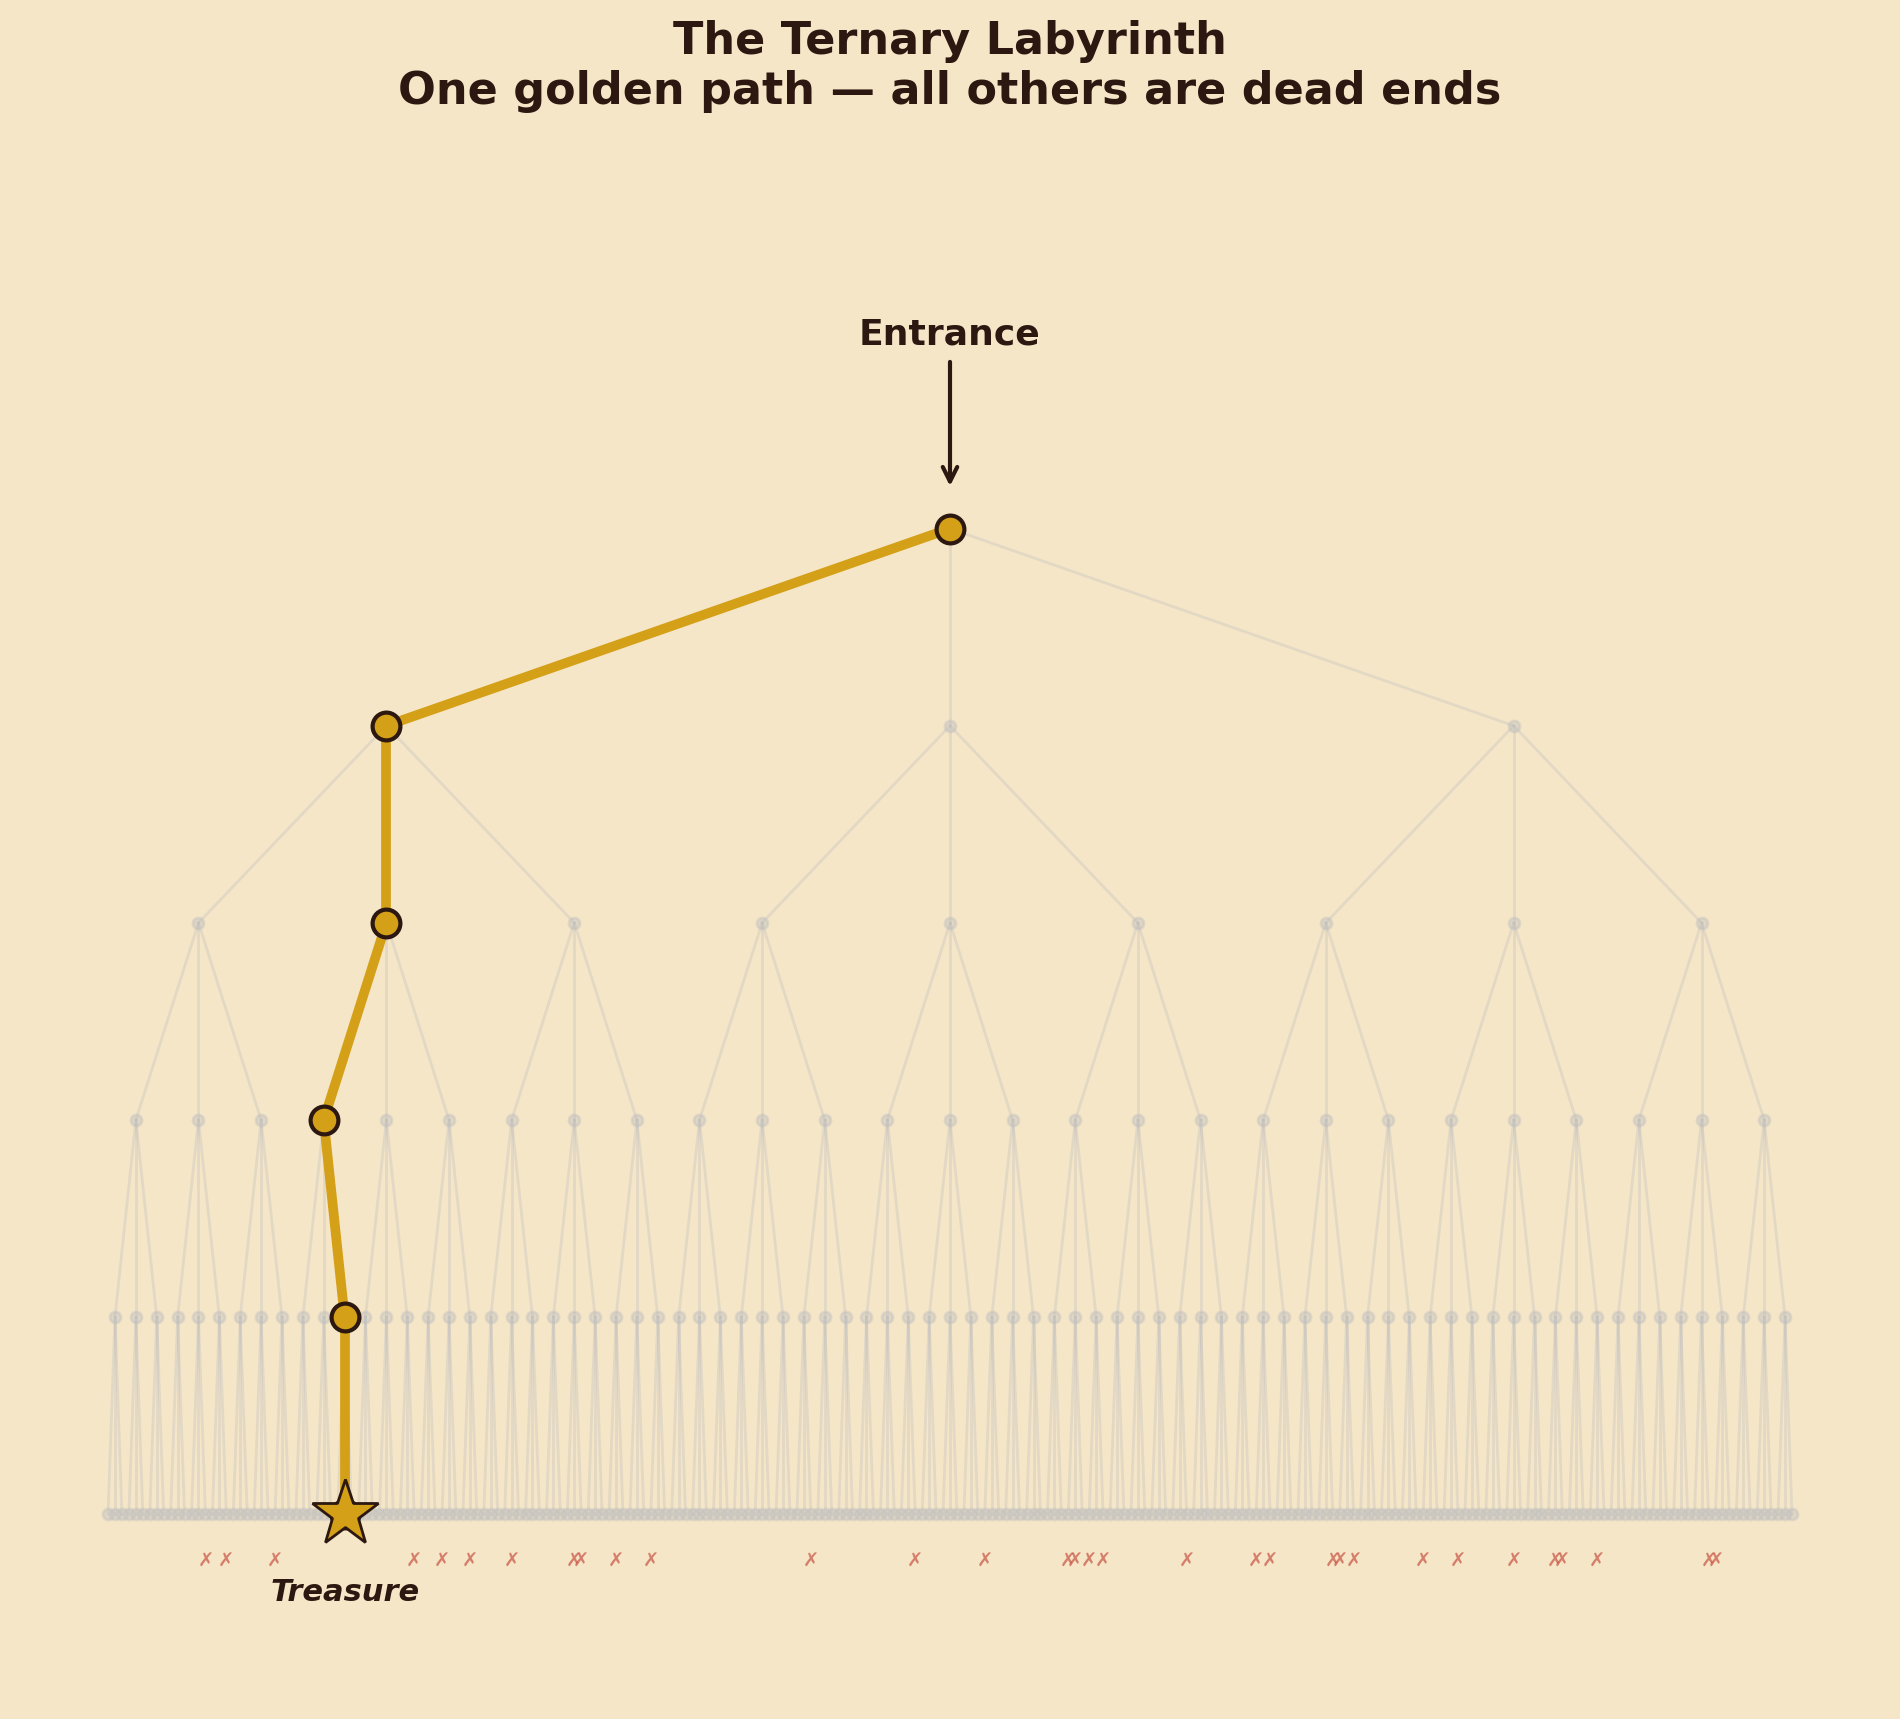
\includegraphics[width=0.82\textwidth]{../Chapter7/images/fig01_ternary_labyrinth.png}
\caption{A stylized cross-section of a ternary labyrinth. At the top, a single entrance leads to a junction that forks into three tunnels, each of which forks into three more, and so on for four or five\ldots}
\end{figure}

\begin{figure}[htbp]
\centering
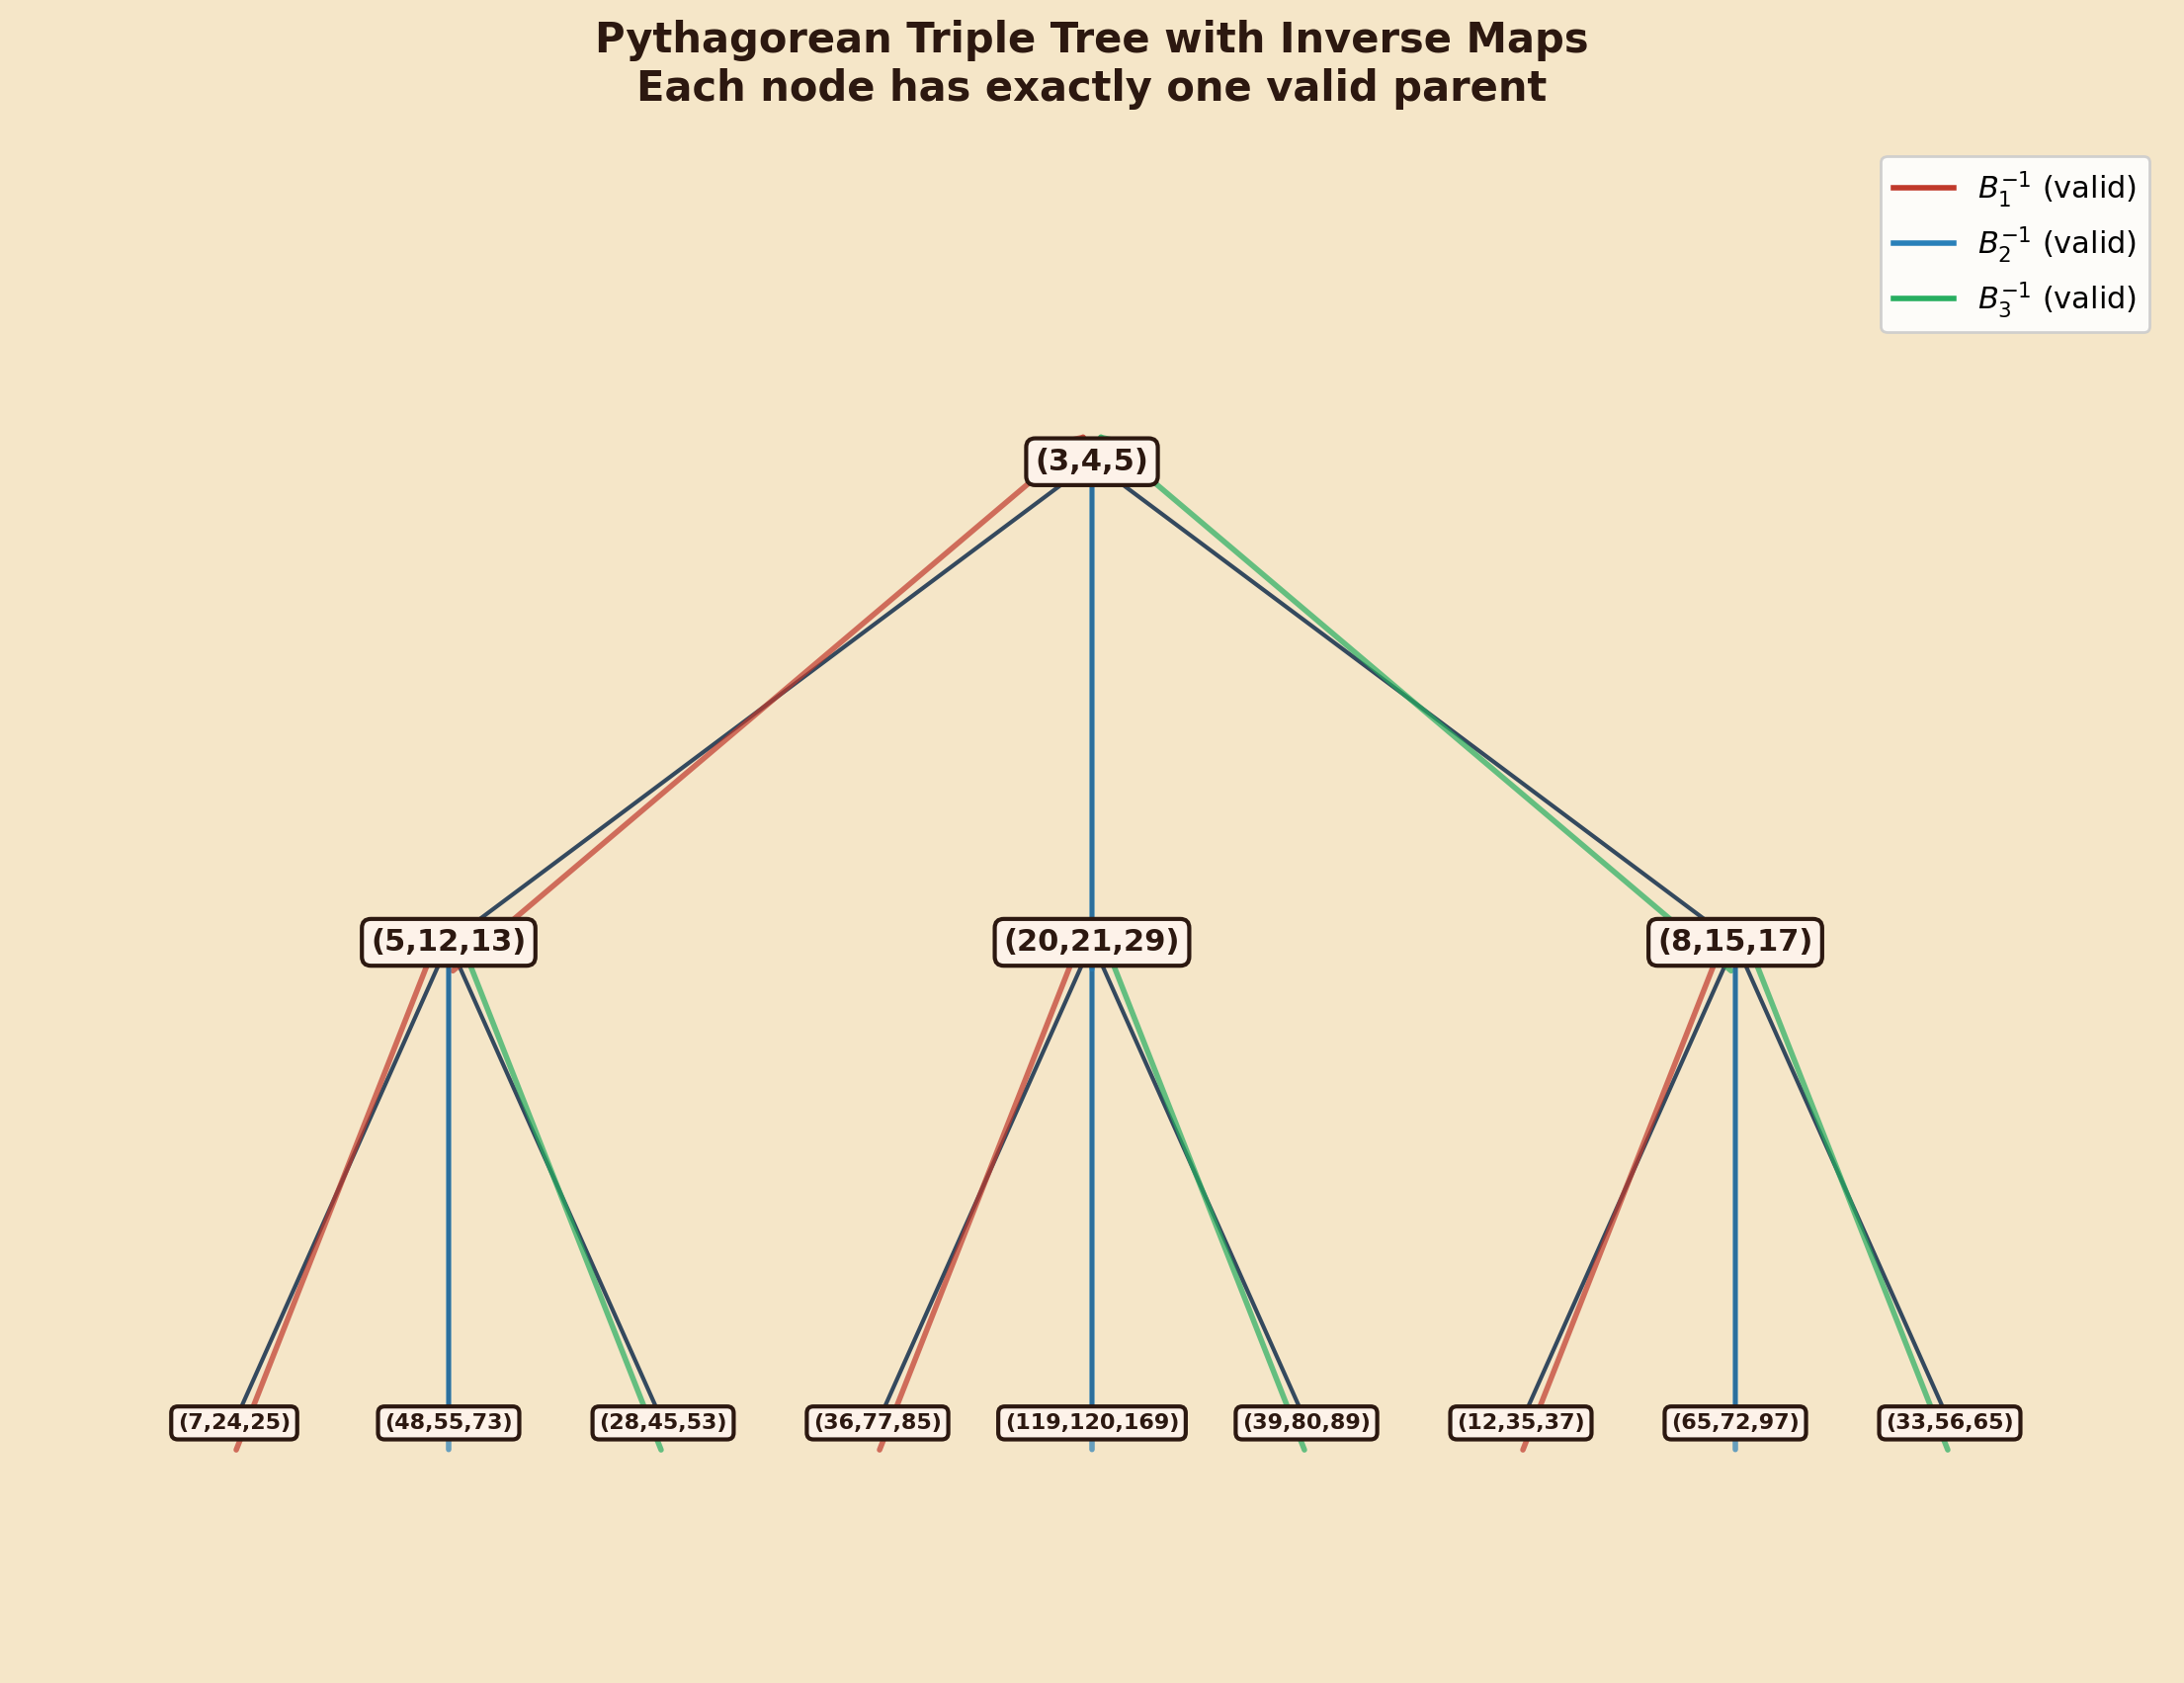
\includegraphics[width=0.82\textwidth]{../Chapter7/images/fig02_triple_tree.png}
\caption{A small portion of the Pythagorean-triple tree, showing the root $(3,4,5)$ and two full levels of branching. Each node is labelled with its triple. Arrows pointing upward (toward the root) are drawn\ldots}
\end{figure}

The question that will occupy us for the rest of this chapter: \textit{can a quantum computer exploit this three-way branching to climb the tree faster?}


\bigskip


\section{The Cancellation Trick}

Here is a small magic trick with negative numbers. Pick any two positive numbers, call them $x$ and $y$. Form the expression $x + y$. It is positive --- obviously. Now form $-x - y$. It is negative --- just as obviously. Notice that their sum is zero:

\[
(x + y) + (-x - y) = 0.
\]

Two quantities that sum to zero cannot both be positive. This observation is so humble it hardly seems worth stating, yet it is the engine behind the entire one-way structure of the Pythagorean tree.

Look closely at the inverse maps. The \textit{second} component of $B_1^{-1}(a, b, c)$ is

\[
s_1 = -2a - b + 2c,
\]

while the second component of $B_2^{-1}(a, b, c)$ is

\[
s_2 = 2a + b - 2c.
\]

Add them:

\[
s_1 + s_2 = (-2a - b + 2c) + (2a + b - 2c) = 0.
\]

If $s_1 > 0$ and $s_2 > 0$, their sum would be positive. But the sum is zero. Contradiction. Therefore $B_1^{-1}(v)$ and $B_2^{-1}(v)$ \textit{cannot both} have all-positive entries.

The same trick disposes of the other two pairs. The \textit{first} components of $B_1^{-1}$ and $B_3^{-1}$ are

\[
f_1 = a + 2b - 2c, \qquad f_3 = -a - 2b + 2c,
\]

and $f_1 + f_3 = 0$. The first components of $B_2^{-1}$ and $B_3^{-1}$ are

\[
f_2 = a + 2b - 2c, \qquad f_3 = -a - 2b + 2c,
\]

and again $f_2 + f_3 = 0$. Three pairs, three cancellations, three impossibilities.

Let us enshrine this as a theorem --- the punchline of the labyrinth.

\begin{quote}
\itshape \textbf{The Determinism Theorem.} *For any integer vector $v = (a, b, c)$ with positive entries, at most one of$B_1^{-1}(v)$, $B_2^{-1}(v)$, $B_3^{-1}(v)$ can have all-positive entries.*
\end{quote}

Define "all-positive" precisely: $\operatorname{pos}(x, y, z) \iff x > 0 \;\wedge\; y > 0 \;\wedge\; z > 0$. The proof is the union of the three two-line arguments above: no pair of inverse images can both satisfy $\operatorname{pos}$, so at most one can.

\[
\operatorname{pos}\!\bigl(B_i^{-1}(v)\bigr) \;\wedge\; \operatorname{pos}\!\bigl(B_j^{-1}(v)\bigr) \;\Longrightarrow\; \text{contradiction}, \quad \text{for all } i \neq j.
\]

The labyrinth has no genuine forks when you are climbing \textit{upward}. Every junction is a one-way corridor.

\begin{figure}[htbp]
\centering
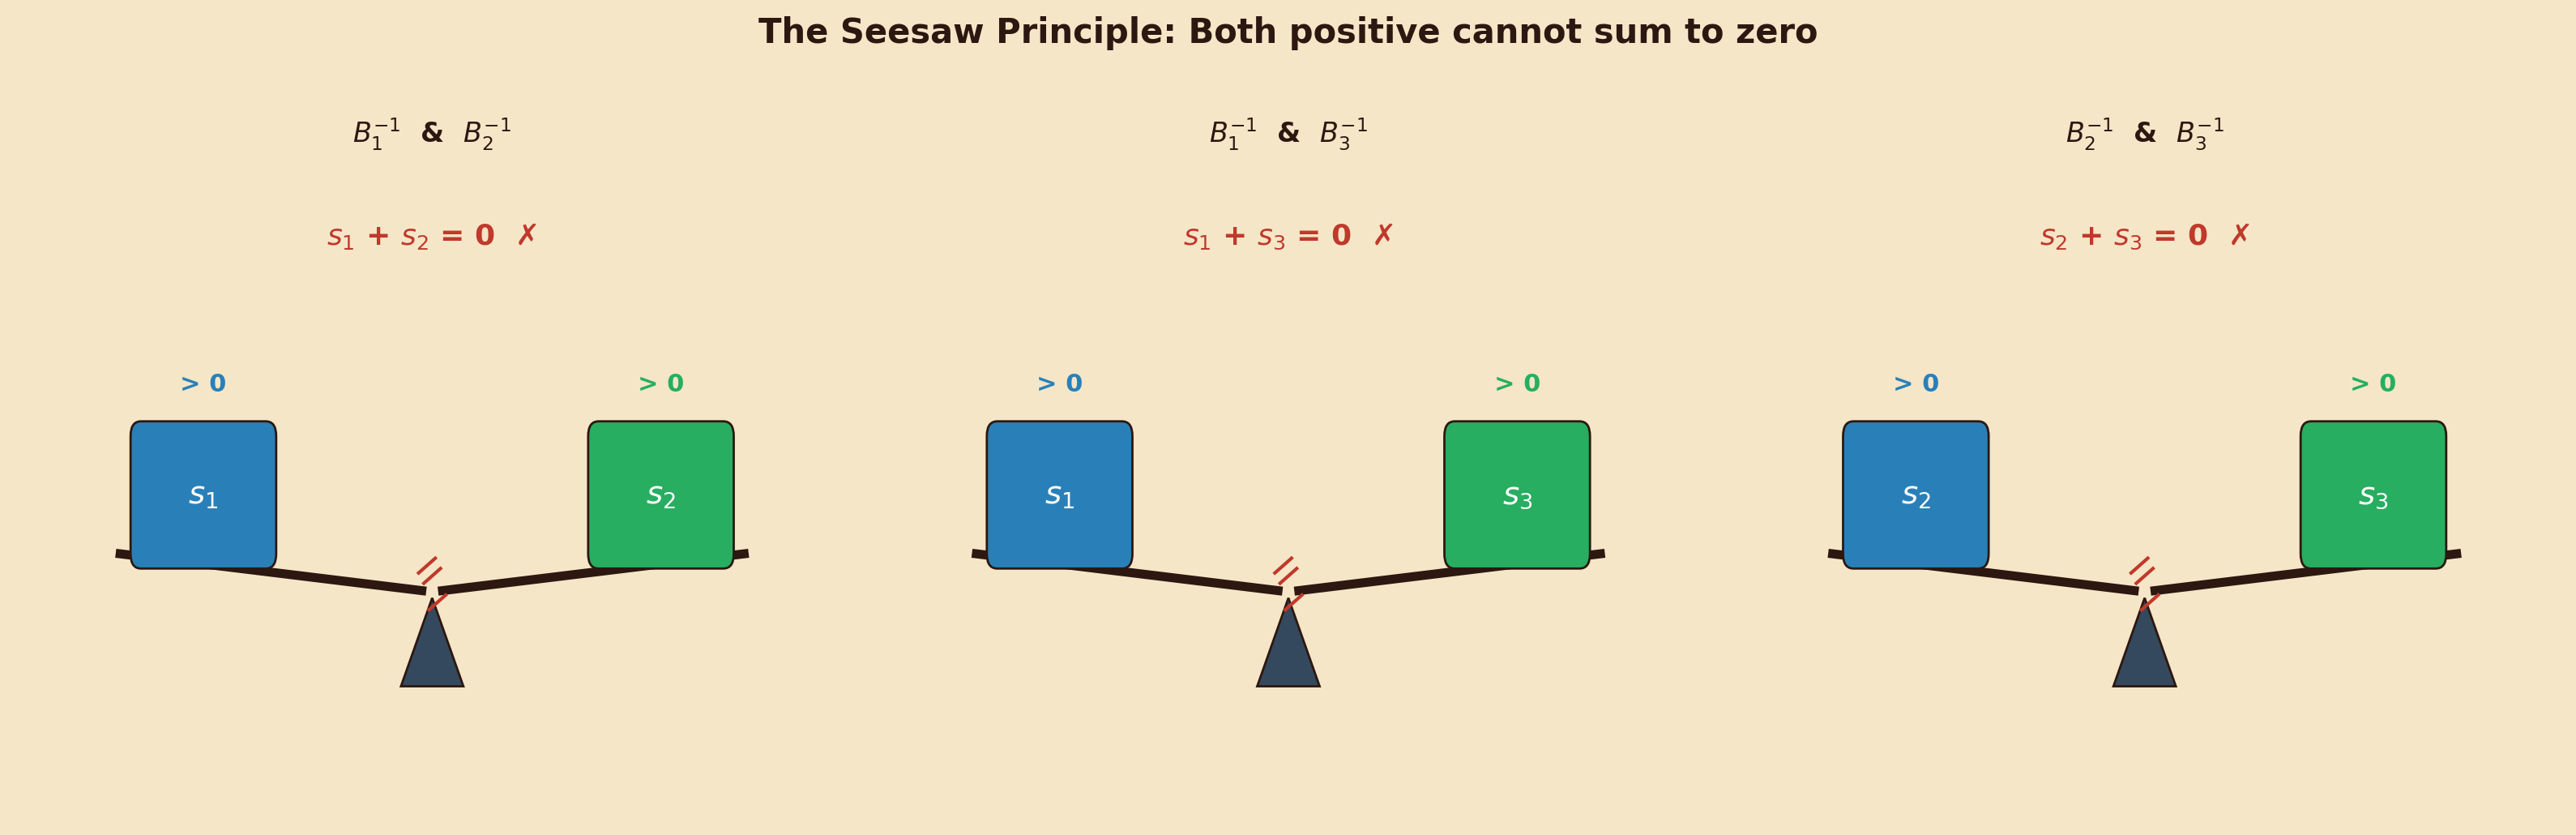
\includegraphics[width=0.82\textwidth]{../Chapter7/images/fig03_seesaw.png}
\caption{A "number-line seesaw" diagram. A horizontal beam is balanced on a fulcrum at zero. On the left side, a weight labelled $s_1$ sits in positive territory; on the right side, a weight labelled $s_2$\ldots}
\end{figure}

\begin{figure}[htbp]
\centering
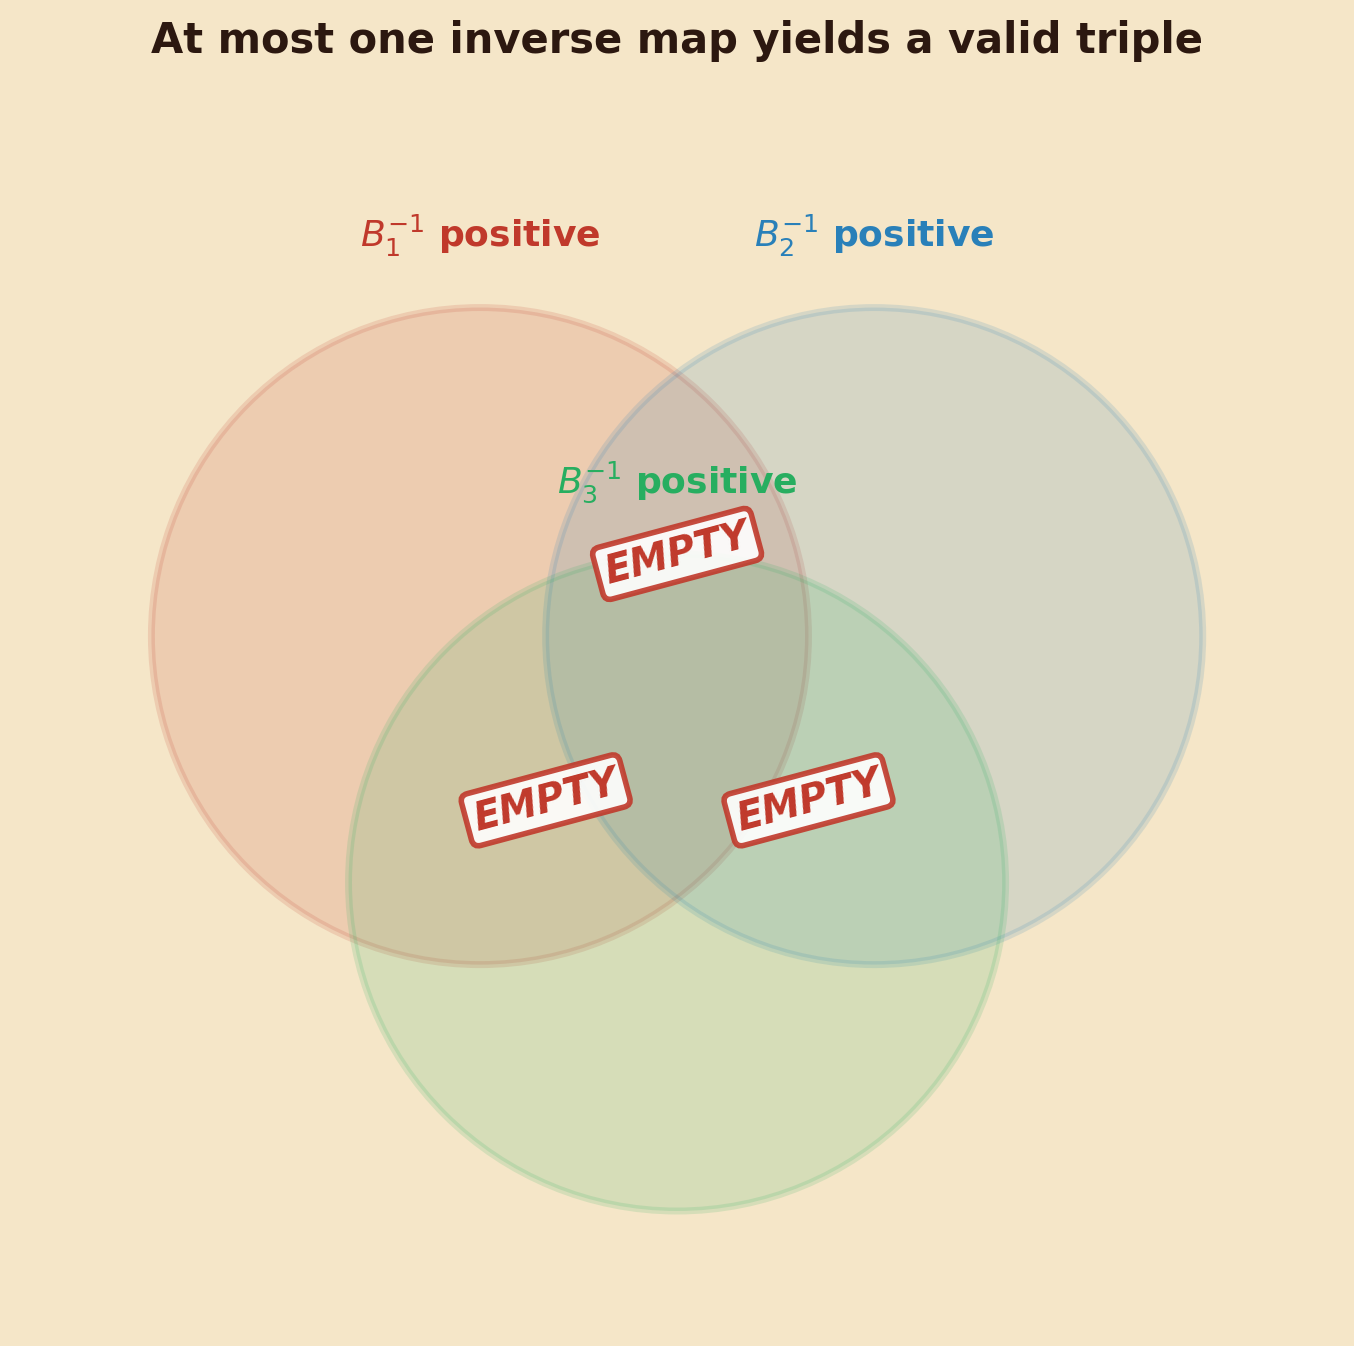
\includegraphics[width=0.82\textwidth]{../Chapter7/images/fig04_venn_exclusive.png}
\caption{A Venn-diagram-style figure with three overlapping circles labelled "$B_1^{-1}$ positive", "$B_2^{-1}$ positive", "$B_3^{-1}$ positive". Every pairwise intersection is shaded and stamped "EMPTY". The\ldots}
\end{figure}


\bigskip


\section{A Parable of the Circular Library}

Before we can understand why the Determinism Theorem defeats the quantum explorer at the forks, we need to understand what quantum computers \textit{actually} do well. The pop-science version --- "they try all answers at once" --- is dangerously misleading, as our labyrinth is about to demonstrate. Let me offer a better parable.

Imagine a circular library with $S$ shelves arranged in a ring. Exactly $M$ of them hold a golden book; the rest hold dust. A classical librarian checks shelves one by one --- on average, she must inspect $S / M$ shelves before finding gold. A quantum librarian can do something genuinely magical: she can query all shelves in \textit{superposition}, then perform a sequence of carefully designed operations that \textit{amplify} the probability of finding a golden shelf while \textit{suppressing} the dusty ones. After roughly $\sqrt{S / M}$ queries --- not $S / M$, but its \textit{square root} --- she measures the system and plucks out a golden book.

This is the essence of Grover's search, discovered by Lov Grover in 1996 and now one of the cornerstones of quantum algorithm design. Stated precisely:

\begin{quote}
\itshape \textbf{Grover's Bound.} *Given a search space of size $S$ containing $M \geq 1$ marked items, there exists a quantum query strategy using at most* $$Q \;\leq\; \left\lfloor \sqrt{\,S / M\,} \right\rfloor + 1$$ \textit{queries that is guaranteed to find a marked item.}
\end{quote}

The square root is remarkable not merely for being faster, but for being \textit{optimal}. Bennett, Bernstein, Brassard, and Vazirani proved shortly after Grover's discovery that $\Omega(\sqrt{S})$ is an unconditional lower bound --- no quantum algorithm, however clever, can search an unstructured space faster. The square root is the speed of light of quantum search: a hard, immovable ceiling.

But notice the crucial qualifier: \textbf{unstructured}. Grover's algorithm helps when you have no better strategy than brute-force checking. If the search space has hidden patterns --- symmetries, monotonicity, algebraic structure --- then entirely different (and sometimes far superior) quantum algorithms may apply. Shor's factoring algorithm, for instance, exploits the \textit{periodic structure} of modular exponentiation, achieving an exponential speedup that Grover's square root cannot match.
\index{Grover!algorithm}

\begin{figure}[htbp]
\centering
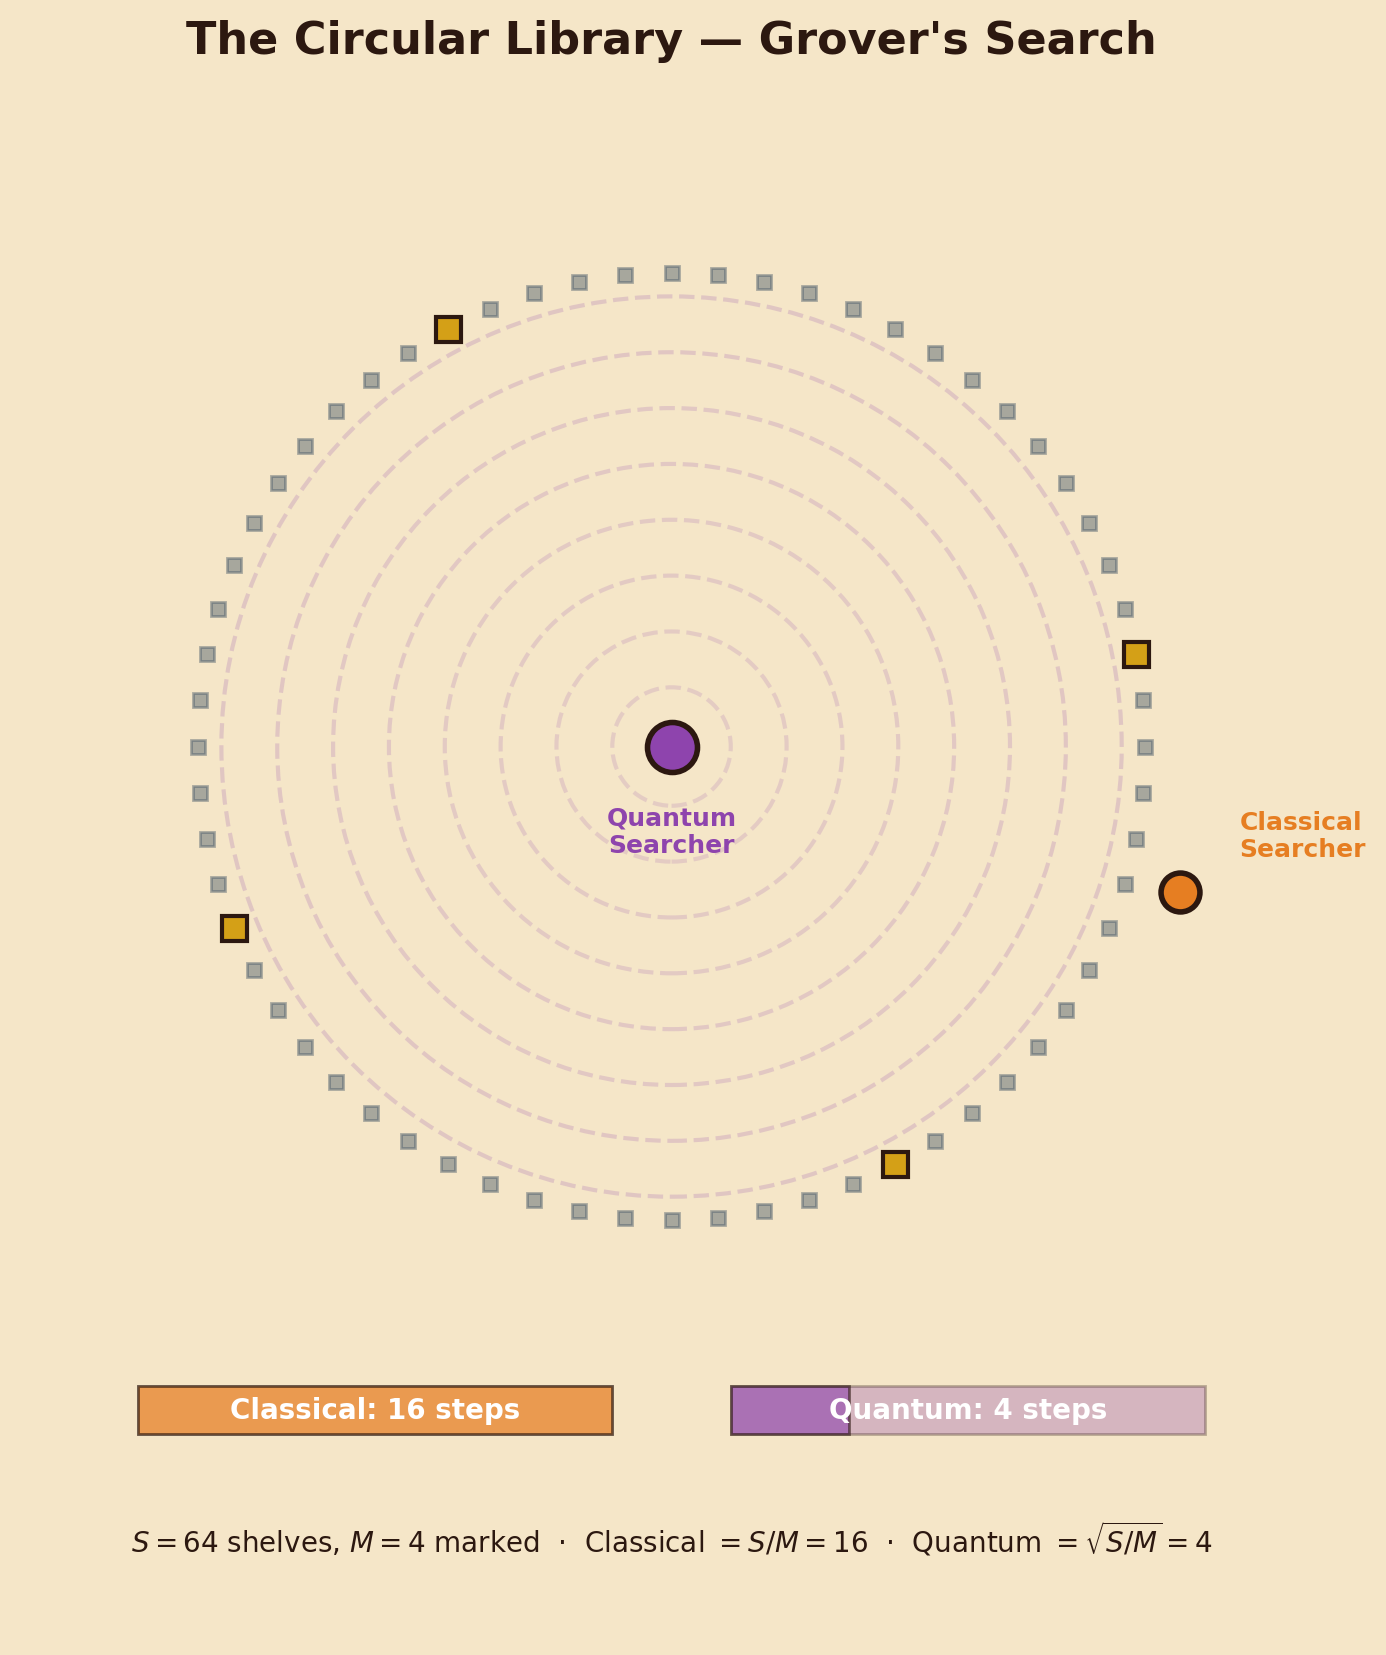
\includegraphics[width=0.82\textwidth]{../Chapter7/images/fig05_circular_library.png}
\caption{The "Circular Library." A bird's-eye view of a ring of $S = 64$ bookshelves arranged in a circle. Four shelves (randomly placed) are coloured gold --- these are the $M = 4$ marked items. A classical\ldots}
\end{figure}


\bigskip


\section{Searching for the Magic Depth}

Now let us return to the Pythagorean tree and the factoring game from earlier chapters. You are handed a large composite number $N$. You build a Pythagorean triple from $N$ --- say, the trivial triple $(N,\; (N^2 - 1)/2,\; (N^2 + 1)/2)$ --- and begin descending toward the root $(3, 4, 5)$, one level at a time. At each level you compute $\gcd(\text{leg},\, N)$. Most levels yield the unhelpful answer $1$ or $N$. But at some critical depth $d^*$, the gcd suddenly spits out a non-trivial factor --- a prime $p$ dividing $N$ --- and the safe swings open.

How deep must you go? That depends on $N$ and its factors, and \textit{you do not know them in advance}. The descent is deterministic --- the Determinism Theorem guarantees a unique path at every junction --- so there is no branching to exploit. The classical cost is simply $d^*$: one gcd computation per level, marching down one level at a time.

Here is where Grover enters --- but through an unexpected door. We cannot use quantum parallelism at the \textit{forks} (there is only one valid path). But we \textit{can} use it along the \textit{depth axis}. Think of the sequence of depths $d = 1, 2, 3, \ldots$ as an unstructured search space. The "marked" item is the depth $d^*$ where the gcd reveals a factor. We do not know $d^*$ in advance --- it could be anywhere from $1$ to $p$ (the smaller prime factor). Grover's algorithm lets us find it in

\[
T_{\text{quantum}} = O\!\left(\sqrt{d^*}\right)
\]

queries, compared to the classical cost of

\[
T_{\text{classical}} = O(d^*).
\]

The speedup is quadratic, not exponential --- but it is genuine, and it comes from the \textit{right} place: the uncertainty of $d^*$, which is genuinely unstructured.

\begin{figure}[htbp]
\centering
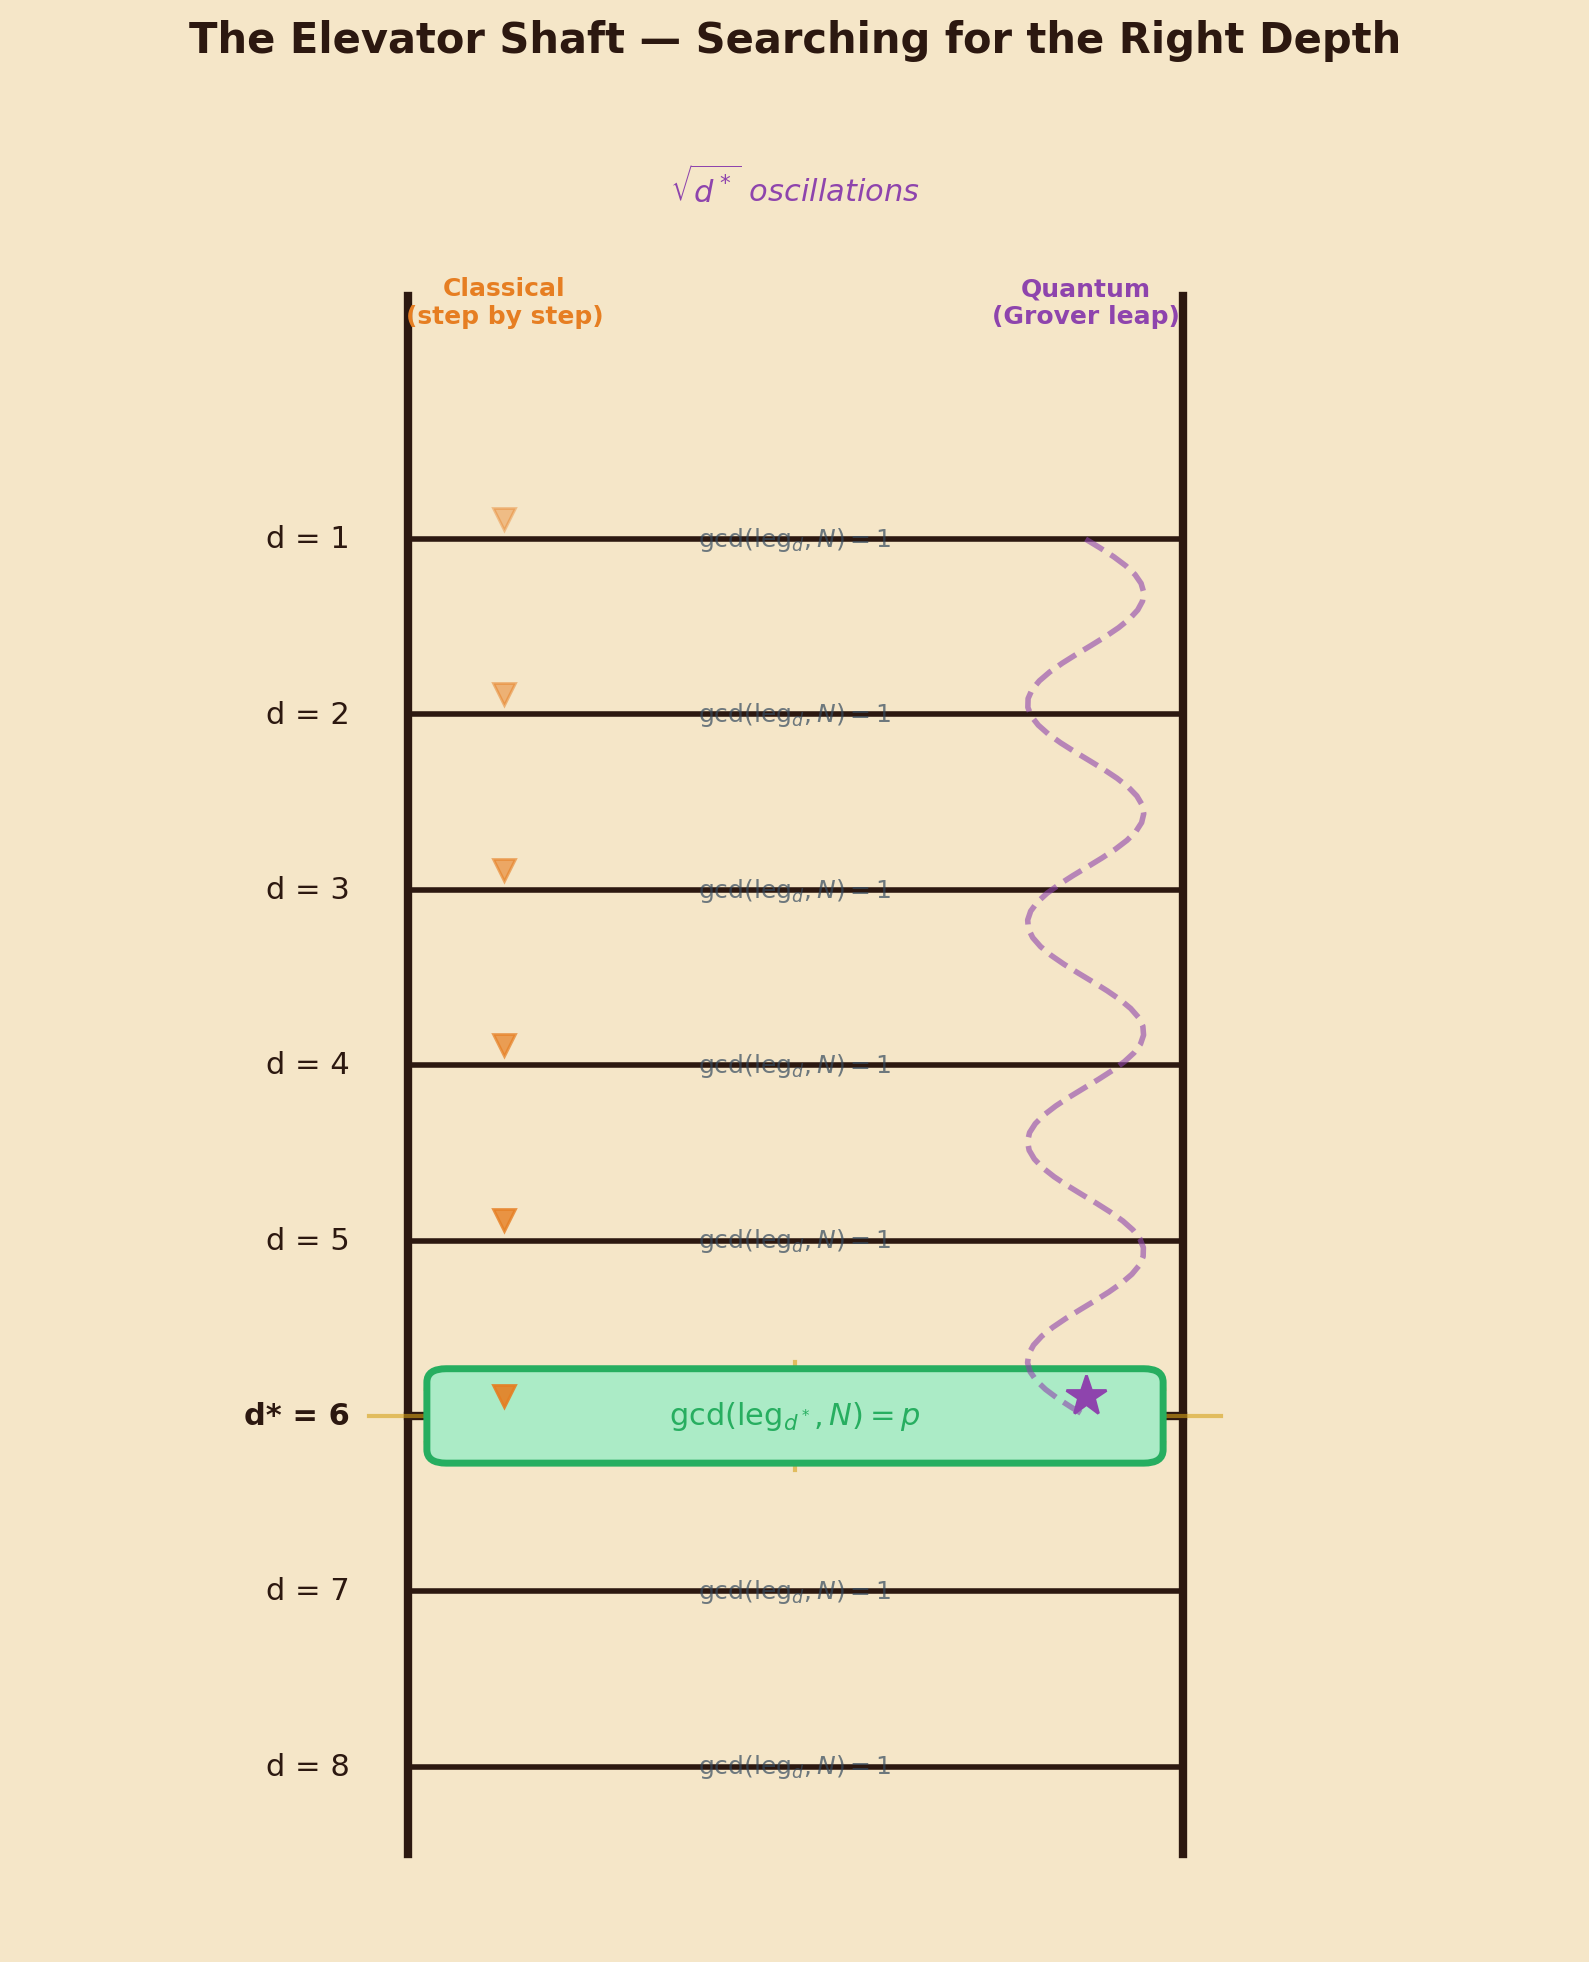
\includegraphics[width=0.82\textwidth]{../Chapter7/images/fig06_elevator_shaft.png}
\caption{A vertical "elevator shaft" diagram. The shaft has floors numbered $d = 1, 2, 3, \ldots, d^*$ from top to bottom. At each floor, a small box shows a gcd computation: "$\gcd(\text{leg}_d,\, N) = 1$"\ldots}
\end{figure}


\bigskip


\section{Balanced Semiprimes and the Fourth-Root Barrier}

A cryptographer builds a lock from the product $N = p \times q$ of two secret primes. If she picks them to be roughly equal --- $p \approx q \approx \sqrt{N}$ --- the number is called a \textit{balanced semiprime}, and it is the bedrock of RSA encryption. How does the critical depth $d^*$ relate to $N$ for these well-balanced locks?
\index{RSA}
\index{semiprime}

The key observation is that $d^* \leq p$: the descent path from the initial triple to the root has length at most $p$, the smaller prime factor. (This bound was established in the analysis of earlier chapters.) For a balanced semiprime, $p \approx \sqrt{N}$. Therefore:

\[
\sqrt{d^*} \;\leq\; \sqrt{p} \;\leq\; \sqrt[4]{p \cdot q} \;=\; N^{1/4}.
\]

The first inequality is the monotonicity of $\sqrt{\cdot}$ applied to $d^* \leq p$. The second uses $p \leq q$, so that $p^2 \leq pq = N$, whence $p \leq \sqrt{N}$ and $\sqrt{p} \leq N^{1/4}$. Let us record this as a theorem:

\begin{quote}
\itshape \textbf{Quantum Balanced Complexity.} *For a balanced semiprime $N = pq$ with $p \leq q$ and critical depth $d^* \leq p$,* $$\sqrt{d^*} \;\leq\; \sqrt{p} \;\leq\; N^{1/4}.$$
\end{quote}

The fourth-root exponent $N^{1/4}$ should ring a bell. It appears in classical fourth-root factoring methods too --- Fermat's method and Lehman's algorithm both achieve $O(N^{1/4})$ complexity by different means. The curious coincidence is that the quantum version of tree descent, exploiting Grover's square root on the depth axis, lands on exactly the same exponent. Different mathematics, same destination.
\index{Fermat!method}
\index{Fermat, Pierre de}

How does this compare to the state of the art? Shor's algorithm, which exploits the \textit{periodic} structure of modular exponentiation, factors $N$ in time $O((\log N)^{2+\varepsilon})$ --- exponentially faster than $N^{1/4}$. For a $1000$-digit number, $N^{1/4}$ has $250$ digits, while $(\log N)^2$ is a modest number in the thousands. Shor wins by a landslide.
\index{Shor!algorithm}

The interest of the $N^{1/4}$ bound lies not in competition with Shor, but in its \textit{provenance}. It arises from tree descent --- a purely geometric-algebraic structure --- rather than from number-theoretic periodicity. It is a different window onto the same landscape.

\begin{figure}[htbp]
\centering
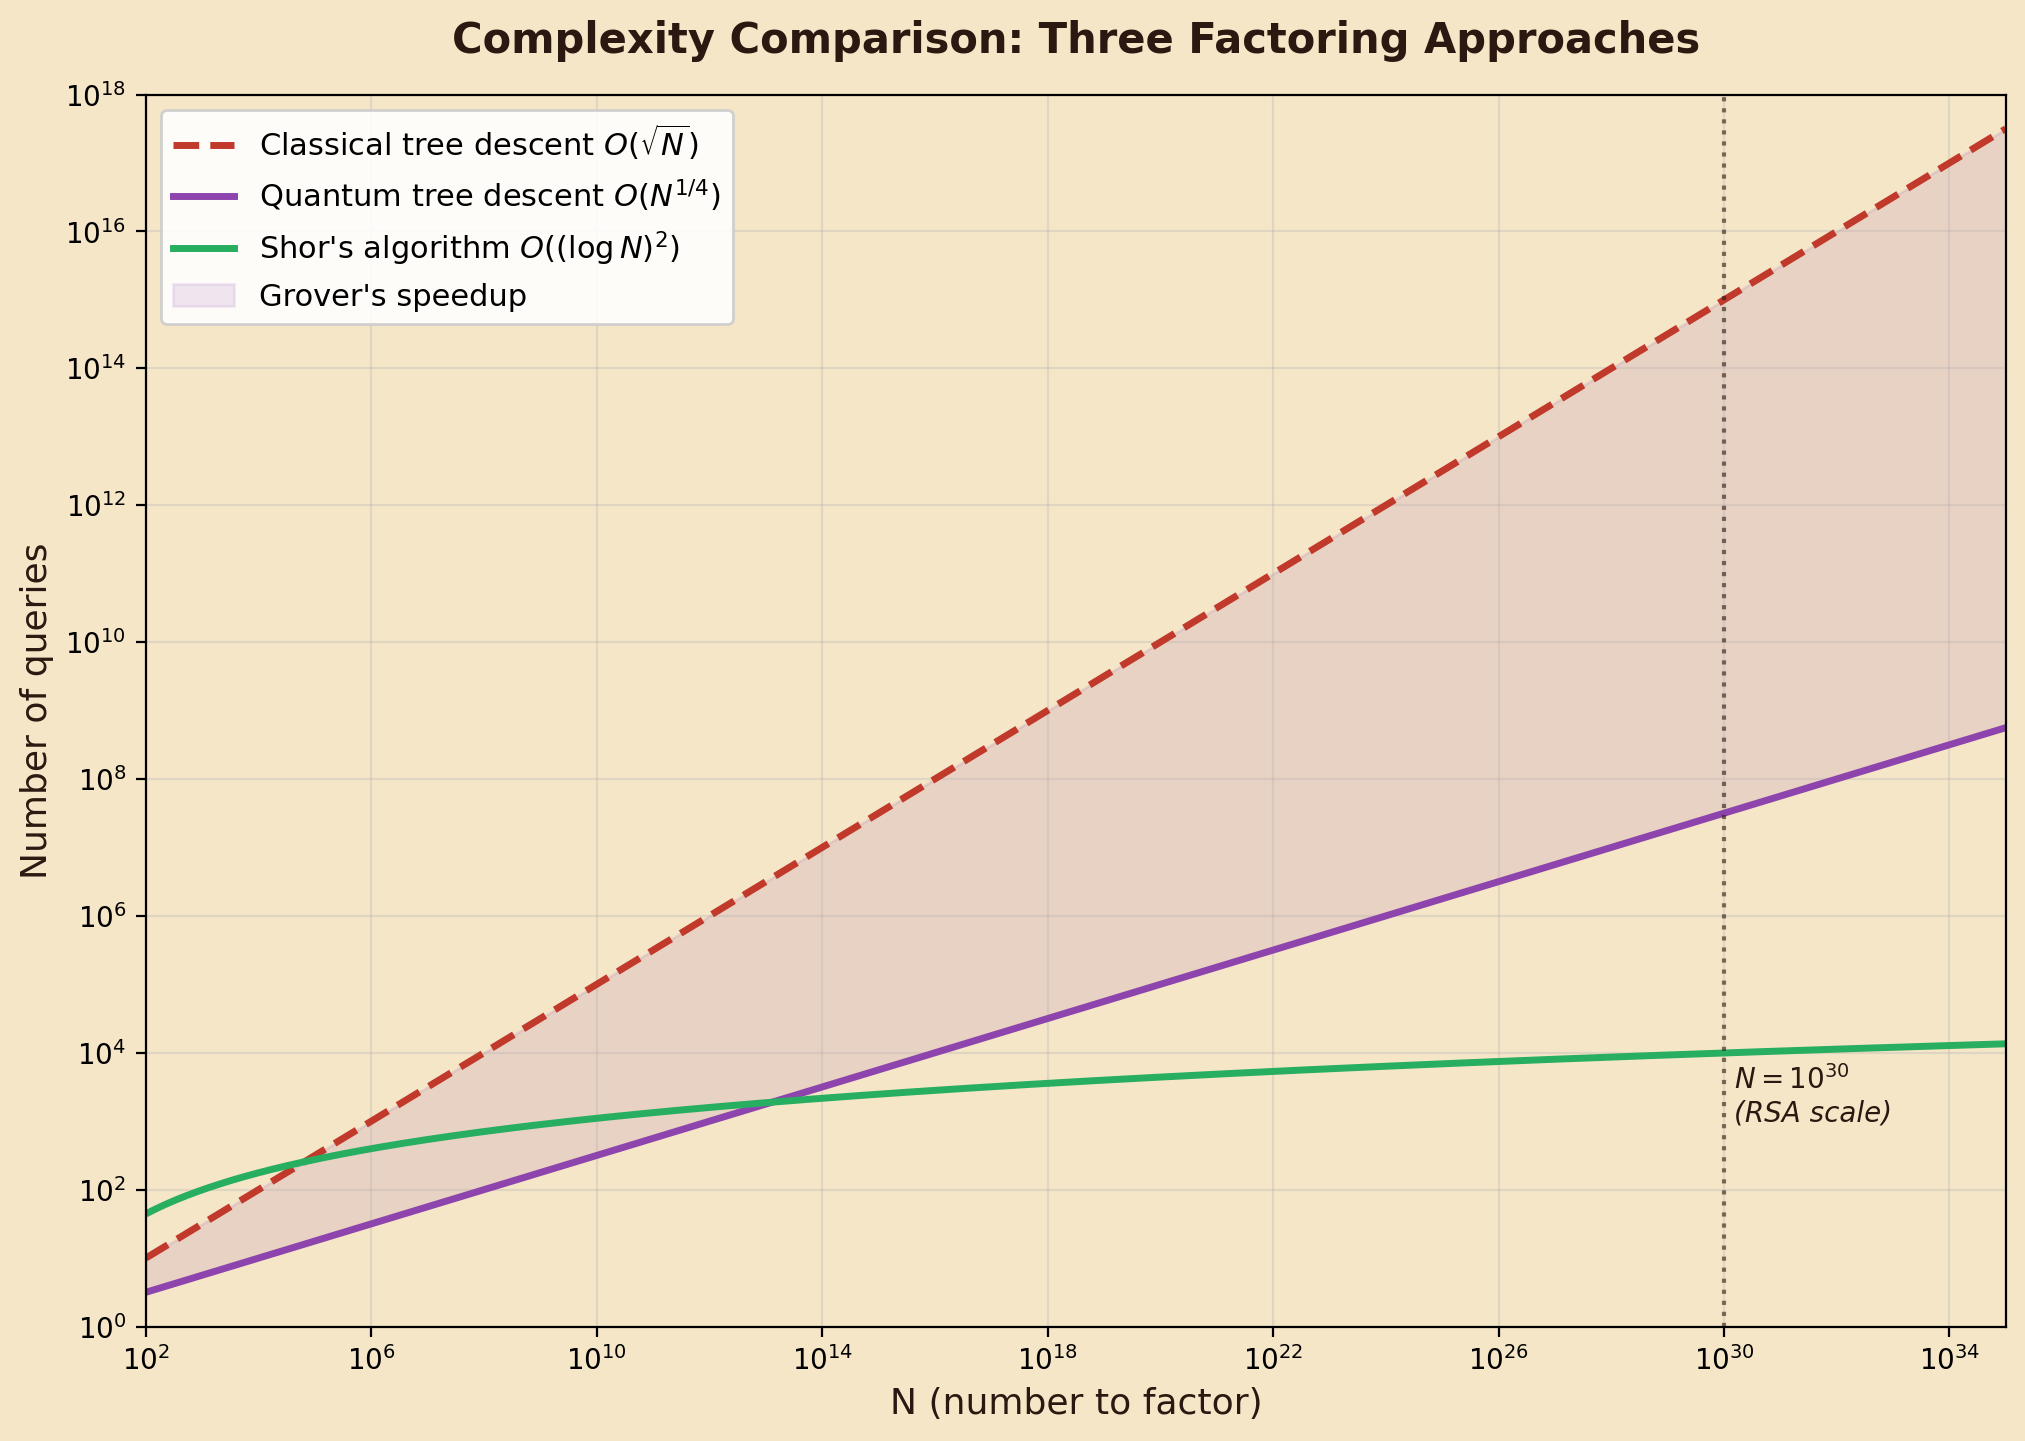
\includegraphics[width=0.82\textwidth]{../Chapter7/images/fig07_complexity_plot.png}
\caption{A log-log plot with $N$ on the horizontal axis and "number of queries" on the vertical axis. Three curves are drawn: (1) $O(\sqrt{N})$ labelled "Classical tree descent," drawn as a steep dashed line.\ldots}
\end{figure}


\bigskip


\section{A Gallery of Dead Ends}

Let us descend together through the tree for a particular number and watch, step by step, as two of the three corridors collapse at every junction.

**Example: $N = 15$.** We form the trivial triple $(15, 112, 113)$ --- check: $15^2 + 112^2 = 225 + 12544 = 12769 = 113^2$. Now apply all three inverse maps:

\[
B_1^{-1}(15, 112, 113) = (15 + 224 - 226,\; -30 - 112 + 226,\; -30 - 224 + 339) = (13, 84, 85).
\]

\[
B_2^{-1}(15, 112, 113) = (15 + 224 - 226,\; 30 + 112 - 226,\; -30 - 224 + 339) = (13, -84, 85).
\]

\[
B_3^{-1}(15, 112, 113) = (-15 - 224 + 226,\; 30 + 112 - 226,\; -30 - 224 + 339) = (-13, -84, 85).
\]

Only $B_1^{-1}$ produces all-positive entries: $(13, 84, 85)$. The other two contain negative entries --- the cancellation trick at work. Exactly one corridor is open.

Check: $\gcd(13, 15) = 1$ and $\gcd(84, 15) = 3$. Already, at the very first descent step, the second leg $84$ shares a factor with $15$. The gcd has betrayed the secret: $3$ is a factor of $15$, and therefore $15 = 3 \times 5$.

The critical depth was $d^* = 1$ --- a single step. Not much for Grover to speed up, but the example beautifully illustrates the mechanism. At every junction, two corridors slam shut; the one that remains open carries the signal that cracks the number.

\begin{figure}[htbp]
\centering
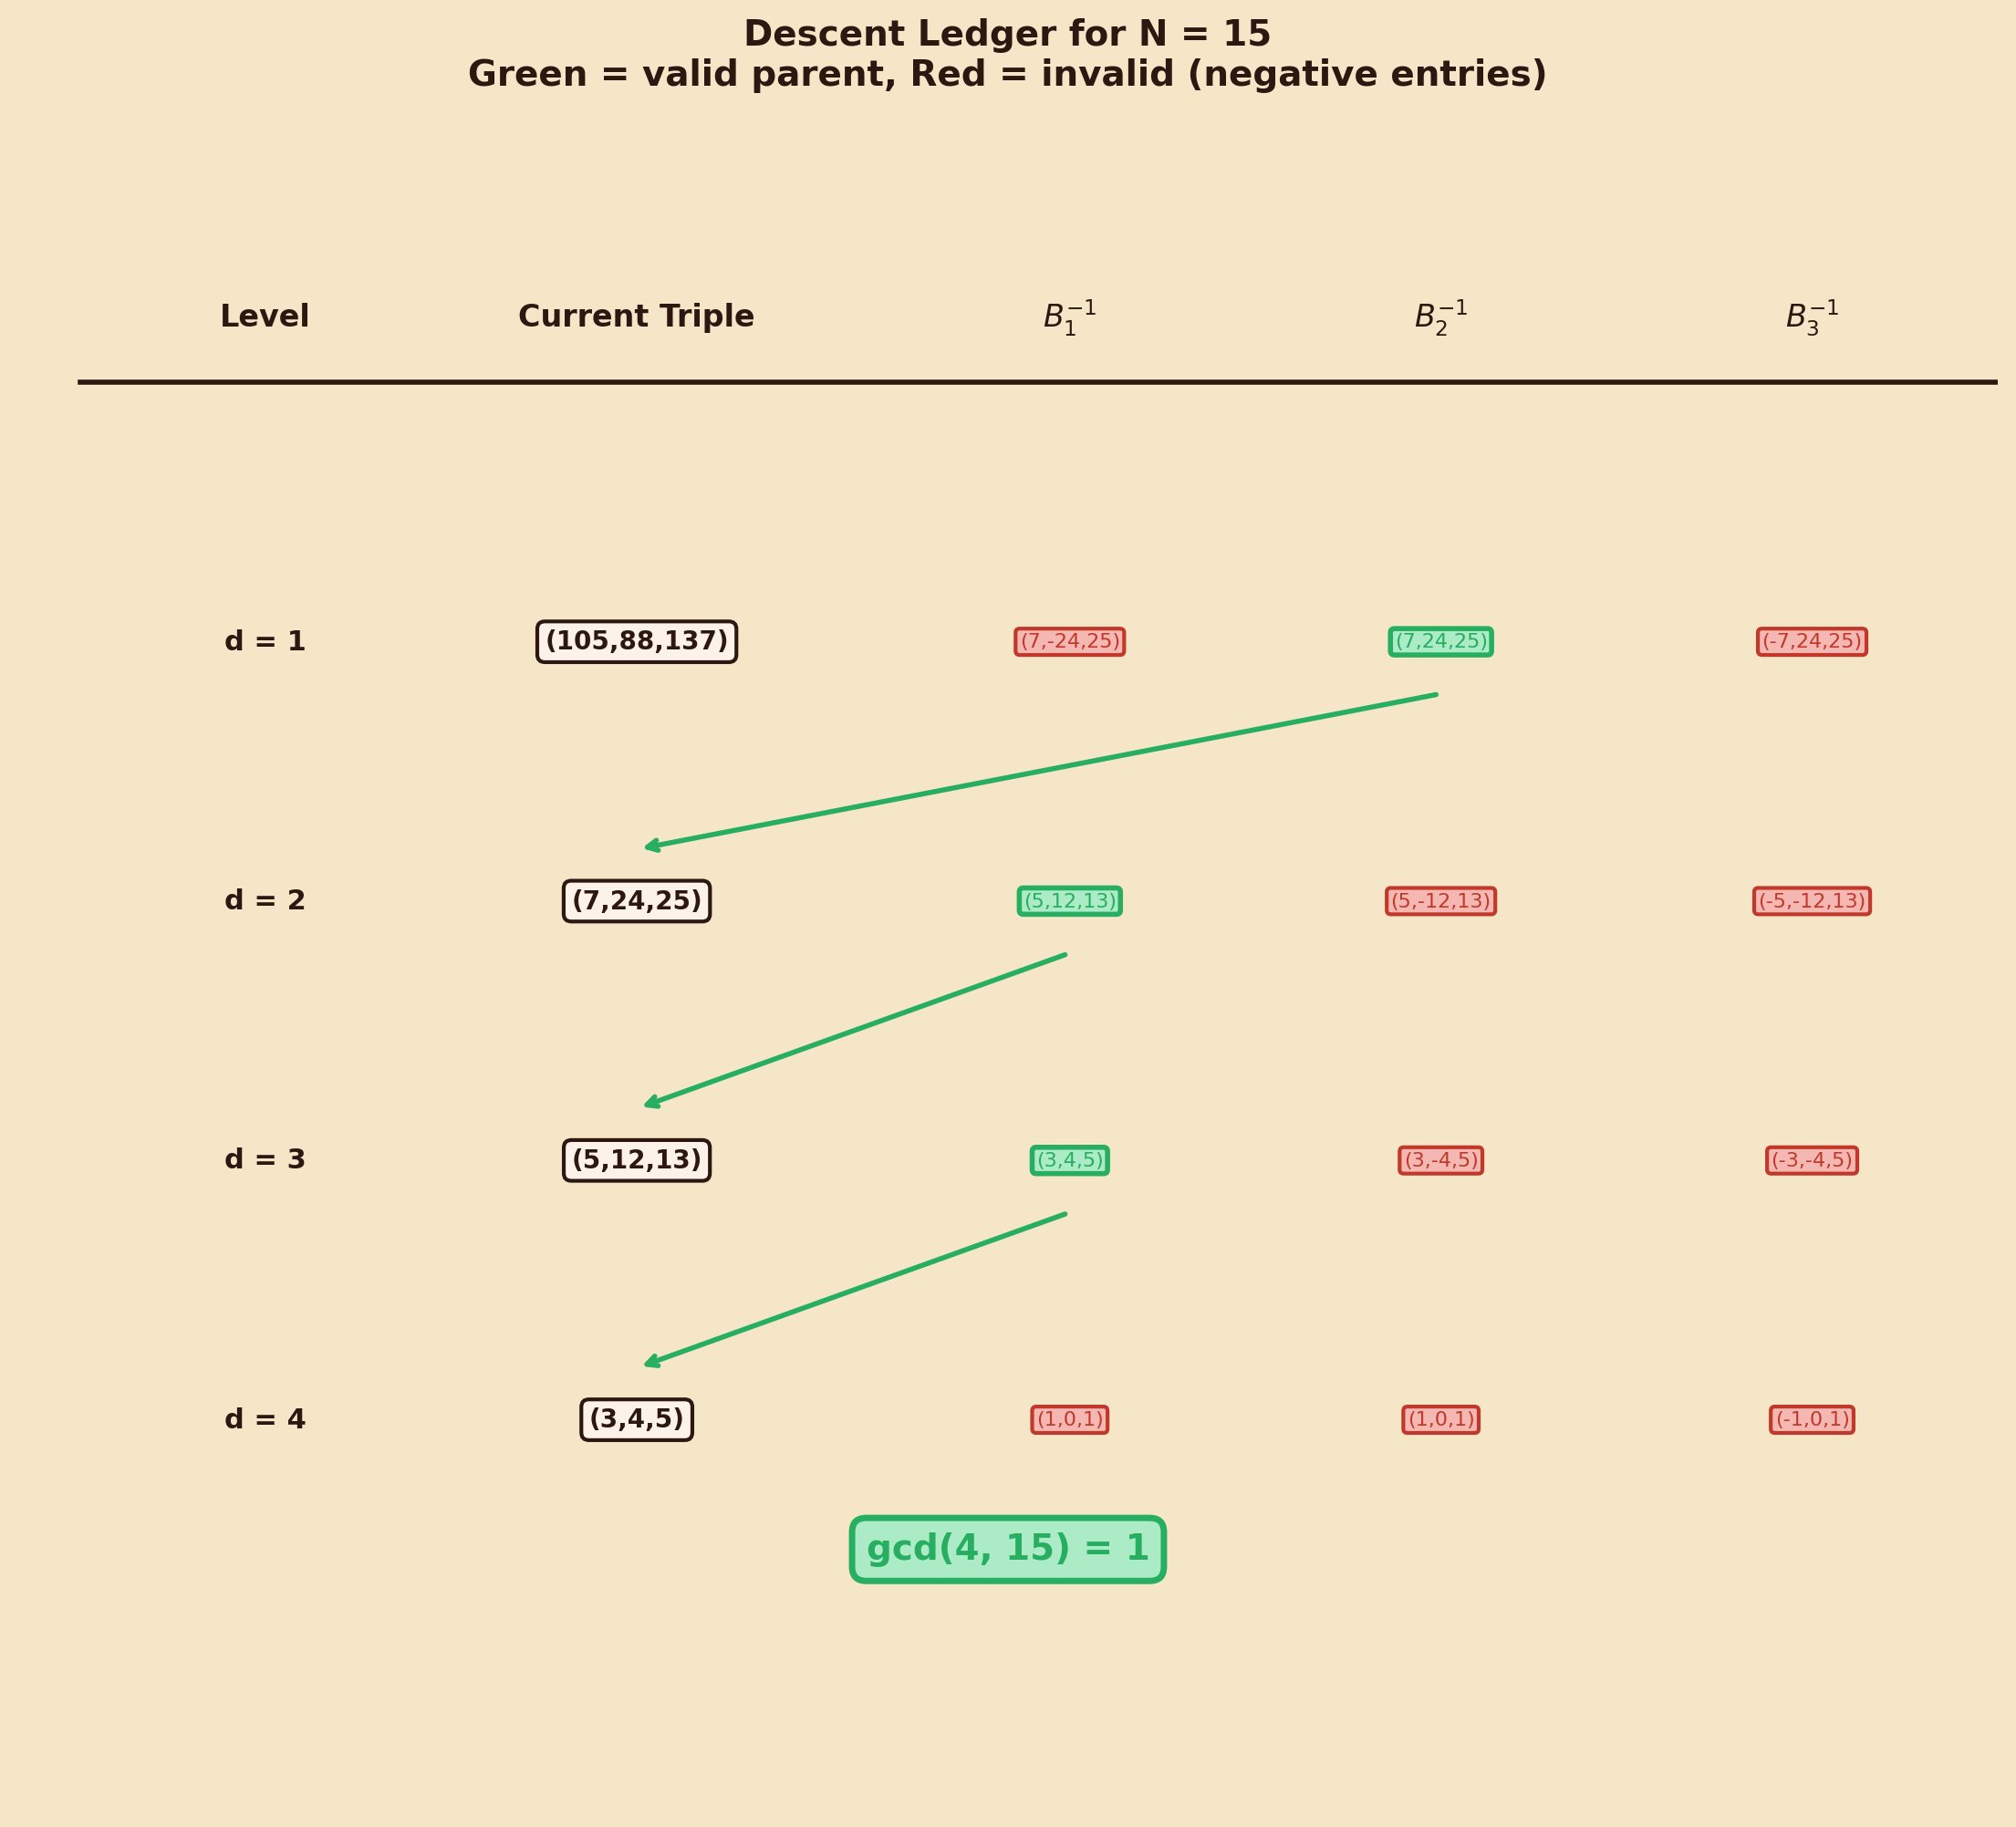
\includegraphics[width=0.82\textwidth]{../Chapter7/images/fig08_descent_ledger.png}
\caption{A "descent ledger" --- a vertical table for $N = 15$. Each row is one level of descent. Three columns show the three candidate parents $B_1^{-1}, B_2^{-1}, B_3^{-1}$. Valid triples (all entries\ldots}
\end{figure}


\bigskip


\section{Why Quantum Parallelism Fails at the Fork}

We have shown that at most one corridor is open at each junction. But wait --- a quantum computer does not \textit{need} the corridor to be physically open. It can explore a superposition of all three corridors simultaneously, and only at the end "measure" to find which one was valid. Surely that helps?

It does not, and the reason is worth savouring, because it cuts to the heart of what quantum speedup really means.

Quantum parallelism is useful when you want to \textit{search} among branches --- when there are many possible answers and you need to find one. Grover's algorithm amplifies the probability of the correct answer through constructive interference, while suppressing wrong answers through destructive interference. But this amplification requires \textit{uncertainty}: there must be multiple plausible candidates for the answer, so that the interference pattern has something to sculpt.

Here, the descent is \textbf{deterministic}. There is exactly one valid path. A quantum computer exploring all three branches in superposition does not gain any advantage, because the "search" has only one candidate and no uncertainty to exploit. It is like reading a novel --- a story with only one plot line is not read faster by a quantum computer. The power of superposition is wasted when there is nothing to interfere with.

Think of it this way. At each junction, a classical computer evaluates one or two inverse maps before finding the positive one --- at worst three evaluations. A quantum computer, using Grover on the three candidates, would need $O(\sqrt{3}) \approx 1.7$ evaluations. You save a fraction of one evaluation per junction --- hardly worth the engineering effort of maintaining quantum coherence.

The \textit{real} quantum opportunity lies elsewhere: along the \textbf{depth axis}. We do not know $d^*$ in advance. The depth levels $d = 1, 2, \ldots$ form a genuinely unstructured search space of size $d^*$, and Grover's algorithm gives a genuine square-root speedup in finding the critical depth. The quantum magic lives not at the forks (which are trivially resolved) but in the \textit{length} of the corridor.

\begin{figure}[htbp]
\centering
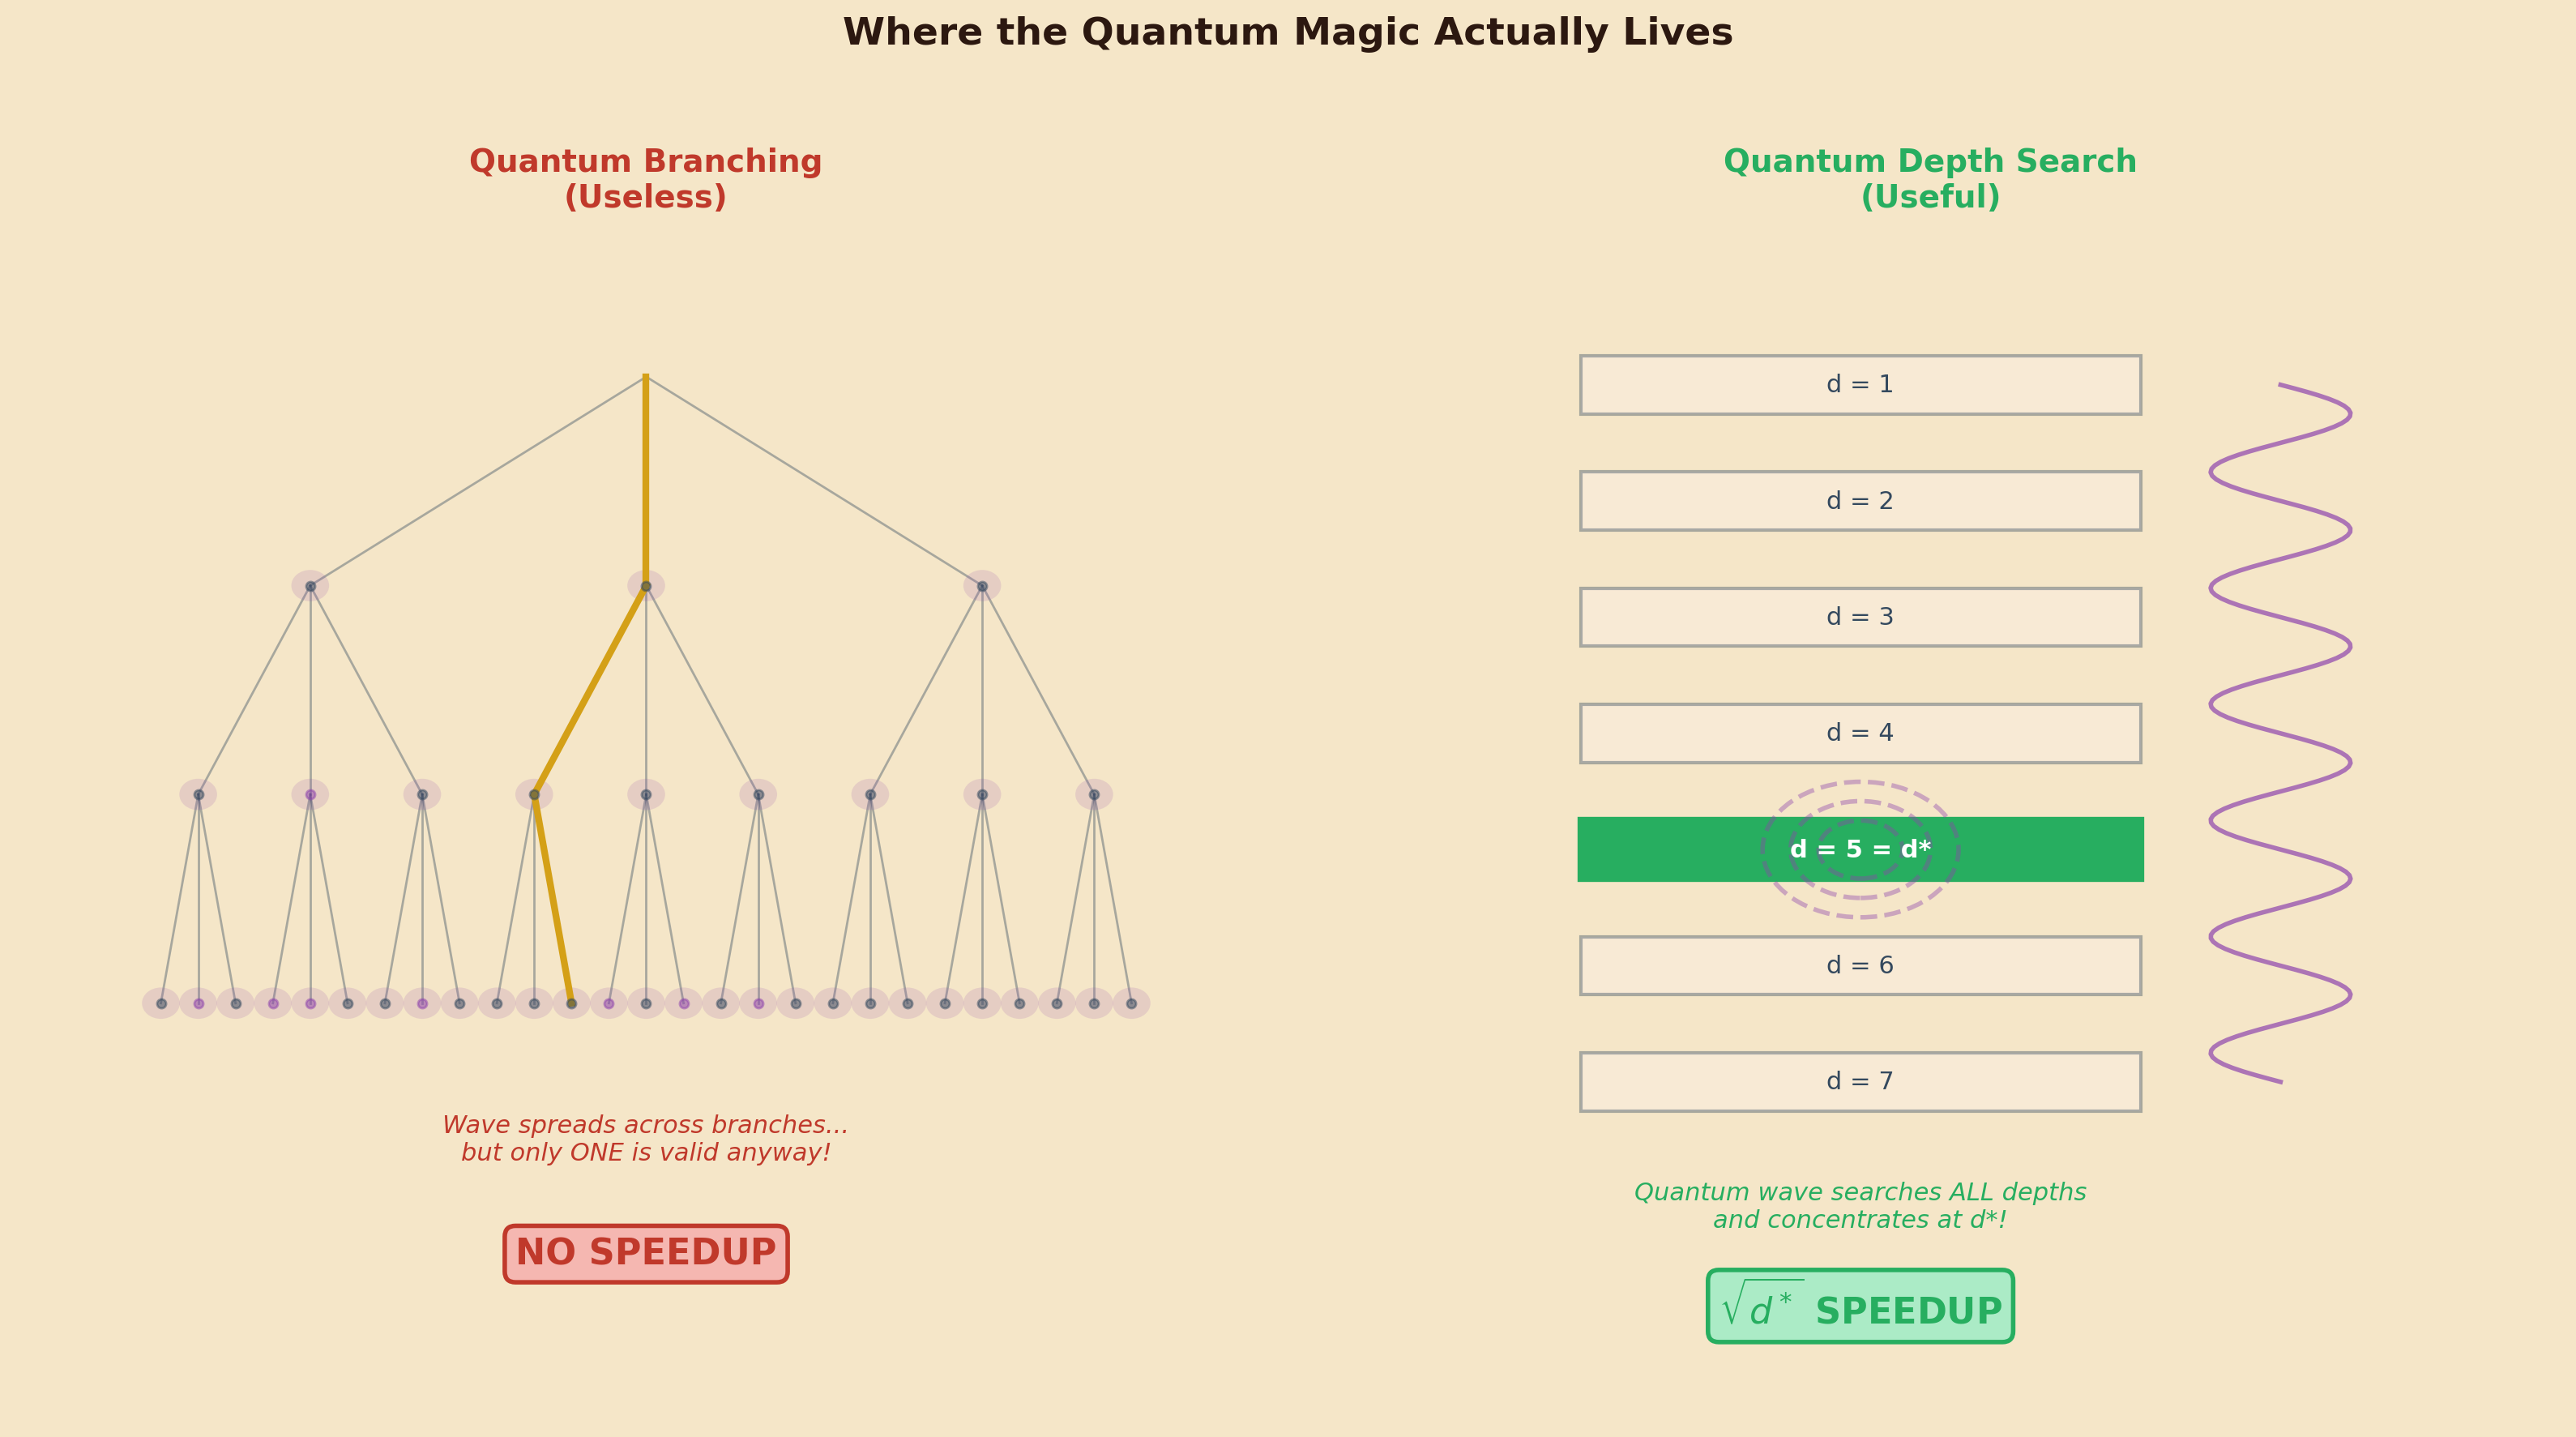
\includegraphics[width=0.82\textwidth]{../Chapter7/images/fig09_maze_solvers.png}
\caption{Two side-by-side "maze solvers." On the left, "Quantum Branching (Useless)": a tree with three branches at each level, one branch highlighted, the quantum wave function shown spreading across all\ldots}
\end{figure}


\bigskip


\section{The Sum-to-Zero Principle}

Here is a puzzle for a rainy afternoon. I give you two functions $f$ and $g$, defined on the same set, and I tell you that $f(x) + g(x) = 0$ for every $x$. What can you deduce?

The answer is immediate: $g = -f$. Wherever $f$ is positive, $g$ is negative, and vice versa. They are mirror images, reflections across the horizontal axis. And crucially: \textit{they can never both be positive at the same point.}

\[
f(x) + g(x) = 0 \;\;\text{for all } x \quad\Longrightarrow\quad \{x : f(x) > 0\} \;\cap\; \{x : g(x) > 0\} = \varnothing.
\]

This is the \textbf{Sum-to-Zero Principle}, and the Determinism Theorem is nothing but three instances of it, applied to the components of the inverse Berggren maps.

The principle is laughably simple, yet it appears --- wearing various disguises --- throughout mathematics and physics. In graph theory, the \textit{handshaking lemma} says that the sum of all vertex degrees equals $2|E|$; the parity constraint that falls out is a Sum-to-Zero argument in disguise. In physics, Newton's third law --- every action has an equal and opposite reaction --- is a sum-to-zero statement about forces. In the theory of \textit{alternating-sign matrices}, the defining property is that the nonzero entries in each row and column alternate in sign and sum to $1$, a condition that creates intricate cancellation patterns governing which entries can be simultaneously positive.

The beauty of the Pythagorean application is its directness. We did not need to invoke any deep theory --- no eigenvalues, no representation theory, no algebraic geometry. The entire one-way structure of the tree, the impossibility of two valid parents, the determinism of the descent --- all of it flows from the observation that certain linear expressions, by their very construction, sum to zero. The simplest tool in the algebraic workshop turned out to be the sharpest.

\begin{figure}[htbp]
\centering
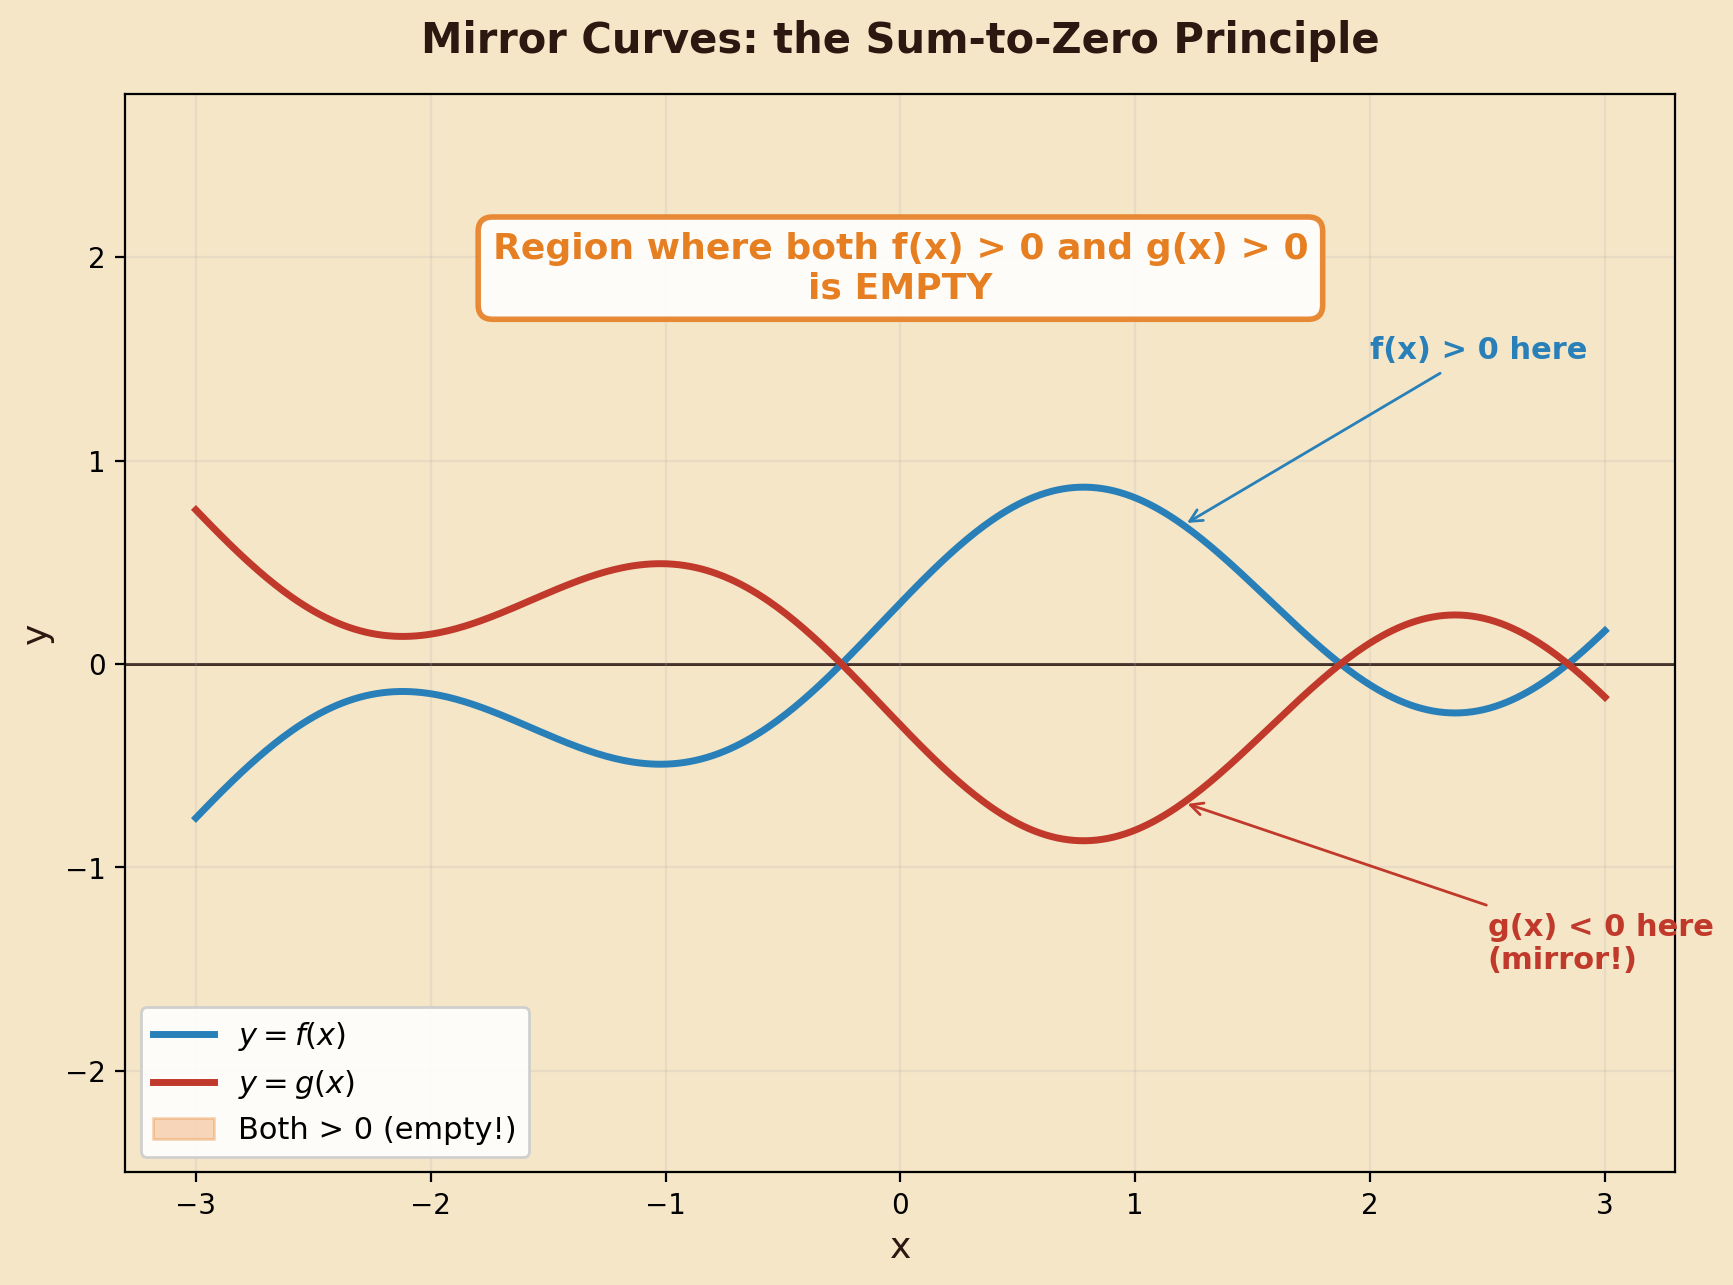
\includegraphics[width=0.82\textwidth]{../Chapter7/images/fig10_mirror_curves.png}
\caption{A coordinate-plane graph. Two curves, $y = f(x)$ (blue) and $y = g(x)$ (red), are plotted. They are exact mirror images across the $x$-axis: wherever blue is above, red is below, and vice versa. The\ldots}
\end{figure}


\bigskip


\section{The Complexity Ladder}

Factoring a number $N$ has a long history of increasingly clever attacks, each shaving away at the exponent. Let us build a \textit{complexity ladder} --- a ranked list of methods, from the most laborious to the most efficient --- and see where our Pythagorean tree descent fits.

At the top of the ladder, the crudest approach: \textbf{trial division}. Test every integer from $2$ up to $\sqrt{N}$. Cost: $O(\sqrt{N})$ divisions. For a $100$-digit number, that is $10^{50}$ operations --- far beyond the capacity of any computer, classical or quantum, that will ever be built.

One rung down: \textbf{classical tree descent}. Build a Pythagorean triple from $N$, descend toward $(3, 4, 5)$, check gcds at each level. For balanced semiprimes, the critical depth satisfies $d^* \leq p \approx \sqrt{N}$, so the cost is $O(\sqrt{N})$ --- the same order as trial division, but with a different constant and a richer algebraic structure.

Another rung: \textbf{quantum tree descent}. Apply Grover's search to the depth axis. Cost: $O(\sqrt{d^*}) \leq O(N^{1/4})$. A quadratic improvement. The key inequality chain:

\[
\sqrt{d^*} \;\leq\; \sqrt{p} \;=\; (p^2)^{1/4} \;\leq\; (pq)^{1/4} \;=\; N^{1/4}.
\]

The first step uses $d^* \leq p$ and monotonicity of $\sqrt{\cdot}$. The second uses $p^2 \leq pq$ (since $p \leq q$). Clean, tight, and elementary.

And at the very bottom of the ladder: \textbf{Shor's algorithm}, which exploits the periodicity of modular exponentiation to factor $N$ in time $O((\log N)^{2+\varepsilon})$. This is not a polynomial improvement --- it is an \textit{exponential} one. For a $1000$-digit number, $(\log N)^2 \approx 10^7$, compared to $N^{1/4} \approx 10^{250}$. Shor's algorithm operates in an entirely different regime.

\begin{center}
\begin{tabular}{c c}
\toprule
Method & Query Complexity \\
\midrule
Trial division & $O(\sqrt{N})$ \\
Classical tree descent & $O(\sqrt{N})$ \\
Quantum tree descent (Grover) & $O(N^{1/4})$ \\
Shor's algorithm & $O((\log N)^{2+\varepsilon})$ \\
\bottomrule
\end{tabular}
\end{center}

Why is the quantum speedup for tree descent "only" quadratic? Because Grover's bound is tight: for unstructured search, $\sqrt{S}$ is the best any quantum algorithm can achieve. And the depth axis is, as far as we know, essentially unstructured --- there is no known pattern in the sequence of depths $d^*$ as a function of $N$ that a quantum algorithm could exploit. The tree descent method, for all its geometric beauty, presents a fundamentally \textit{unstructured} search problem to the quantum computer, and Grover's square-root ceiling applies without exception.

\begin{figure}[htbp]
\centering
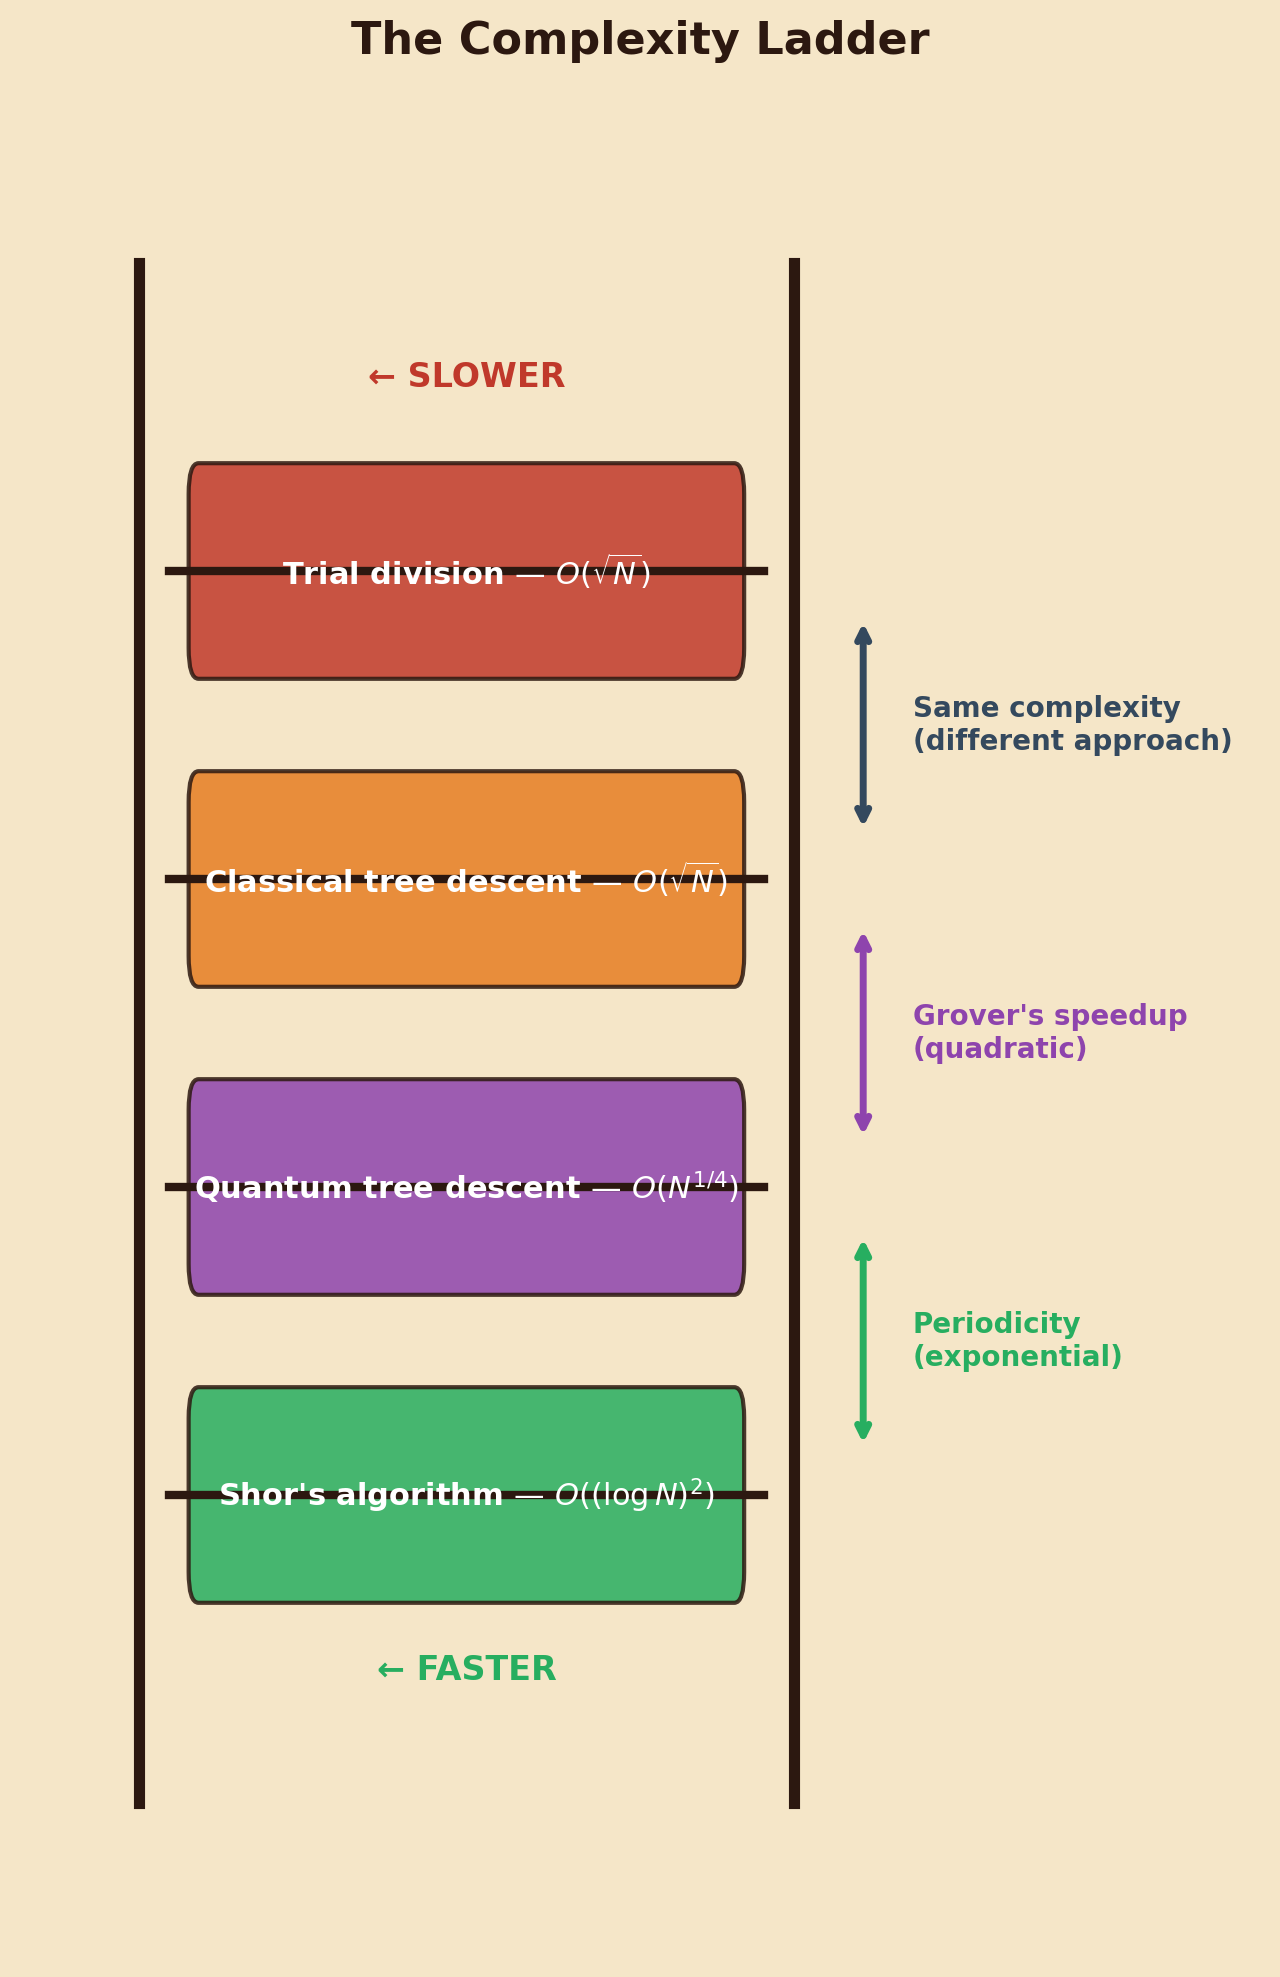
\includegraphics[width=0.82\textwidth]{../Chapter7/images/fig11_complexity_ladder.png}
\caption{A vertical "ladder" diagram. Each rung is labelled with a factoring method and its complexity exponent. The bottom rung (fastest) is Shor at $O((\log N)^2)$. The next rung up is Quantum tree descent\ldots}
\end{figure}


\bigskip


\section{Open Corridors}

Every good chapter of mathematics should end not with a period but with a question mark. We have mapped the one-way corridors of the Pythagorean tree and measured them with quantum rulers. The central surprise --- that the labyrinth's branching structure is trivial while the \textit{depth} is the true search problem --- is both a specific theorem about Pythagorean triples and a parable about quantum computing. But several doors remain locked. Let me leave you with the ones I find most tantalising.

\textbf{The existence question.} We proved that \textit{at most one} branch is valid at each junction. But must \textit{at least one} always be valid for every non-root primitive triple? This is the companion "existence" half of the Determinism Theorem. Together, "at most one" and "at least one" yield "exactly one" --- the statement that the descent path is not merely unique but \textit{guaranteed to exist}. What would a self-contained proof of this stronger claim look like?

\textbf{Structured depth.} We treated the depth axis as unstructured --- a featureless sequence of levels, with no pattern to exploit. But is it really featureless? Could the arithmetic of the descent --- the specific way the Berggren matrices transform the legs of the triple --- give \textit{additional structure} that a quantum algorithm could exploit beyond Grover? Could $d^*$ be predicted, even approximately, from number-theoretic properties of $N$?

\textbf{Multi-channel Grover.} Chapter 6 introduced higher $k$-tuple extensions with multiple independent gcd channels --- seven keyholes instead of one. If we run Grover searches on $k$ channels simultaneously, does the combined success probability improve? The channels are independent, so their amplitudes might interfere constructively. But independence can also mean that no single channel benefits from the others. The analysis is open.

\textbf{Hybrid algorithms.} A practical protocol might combine classical descent (cheap per step, requiring no quantum coherence) with intermittent quantum depth probes (expensive per step, but covering many levels at once). What is the optimal interleaving? This is a question in the theory of \textit{hybrid quantum-classical algorithms}, a rapidly developing field where the boundary between quantum advantage and classical efficiency is still poorly understood.

\textbf{Physical realisability.} Grover's algorithm requires maintaining coherent superposition over $d^*$ depth levels. For an RSA-scale number $N \sim 10^{300}$, the smaller prime factor is $p \sim 10^{150}$, and the critical depth could be as large as $d^* \sim 10^{150}$. A quantum computer would need to maintain superposition over $10^{150}$ levels --- a number so vast that even the most optimistic projections of quantum hardware fall short by a hundred orders of magnitude. The $N^{1/4}$ bound is a mathematical truth; whether it is a \textit{physical} possibility is another matter entirely.

These questions are corridors that stretch into the distance, each one forking and branching in its own right. The labyrinth continues.

\begin{figure}[htbp]
\centering
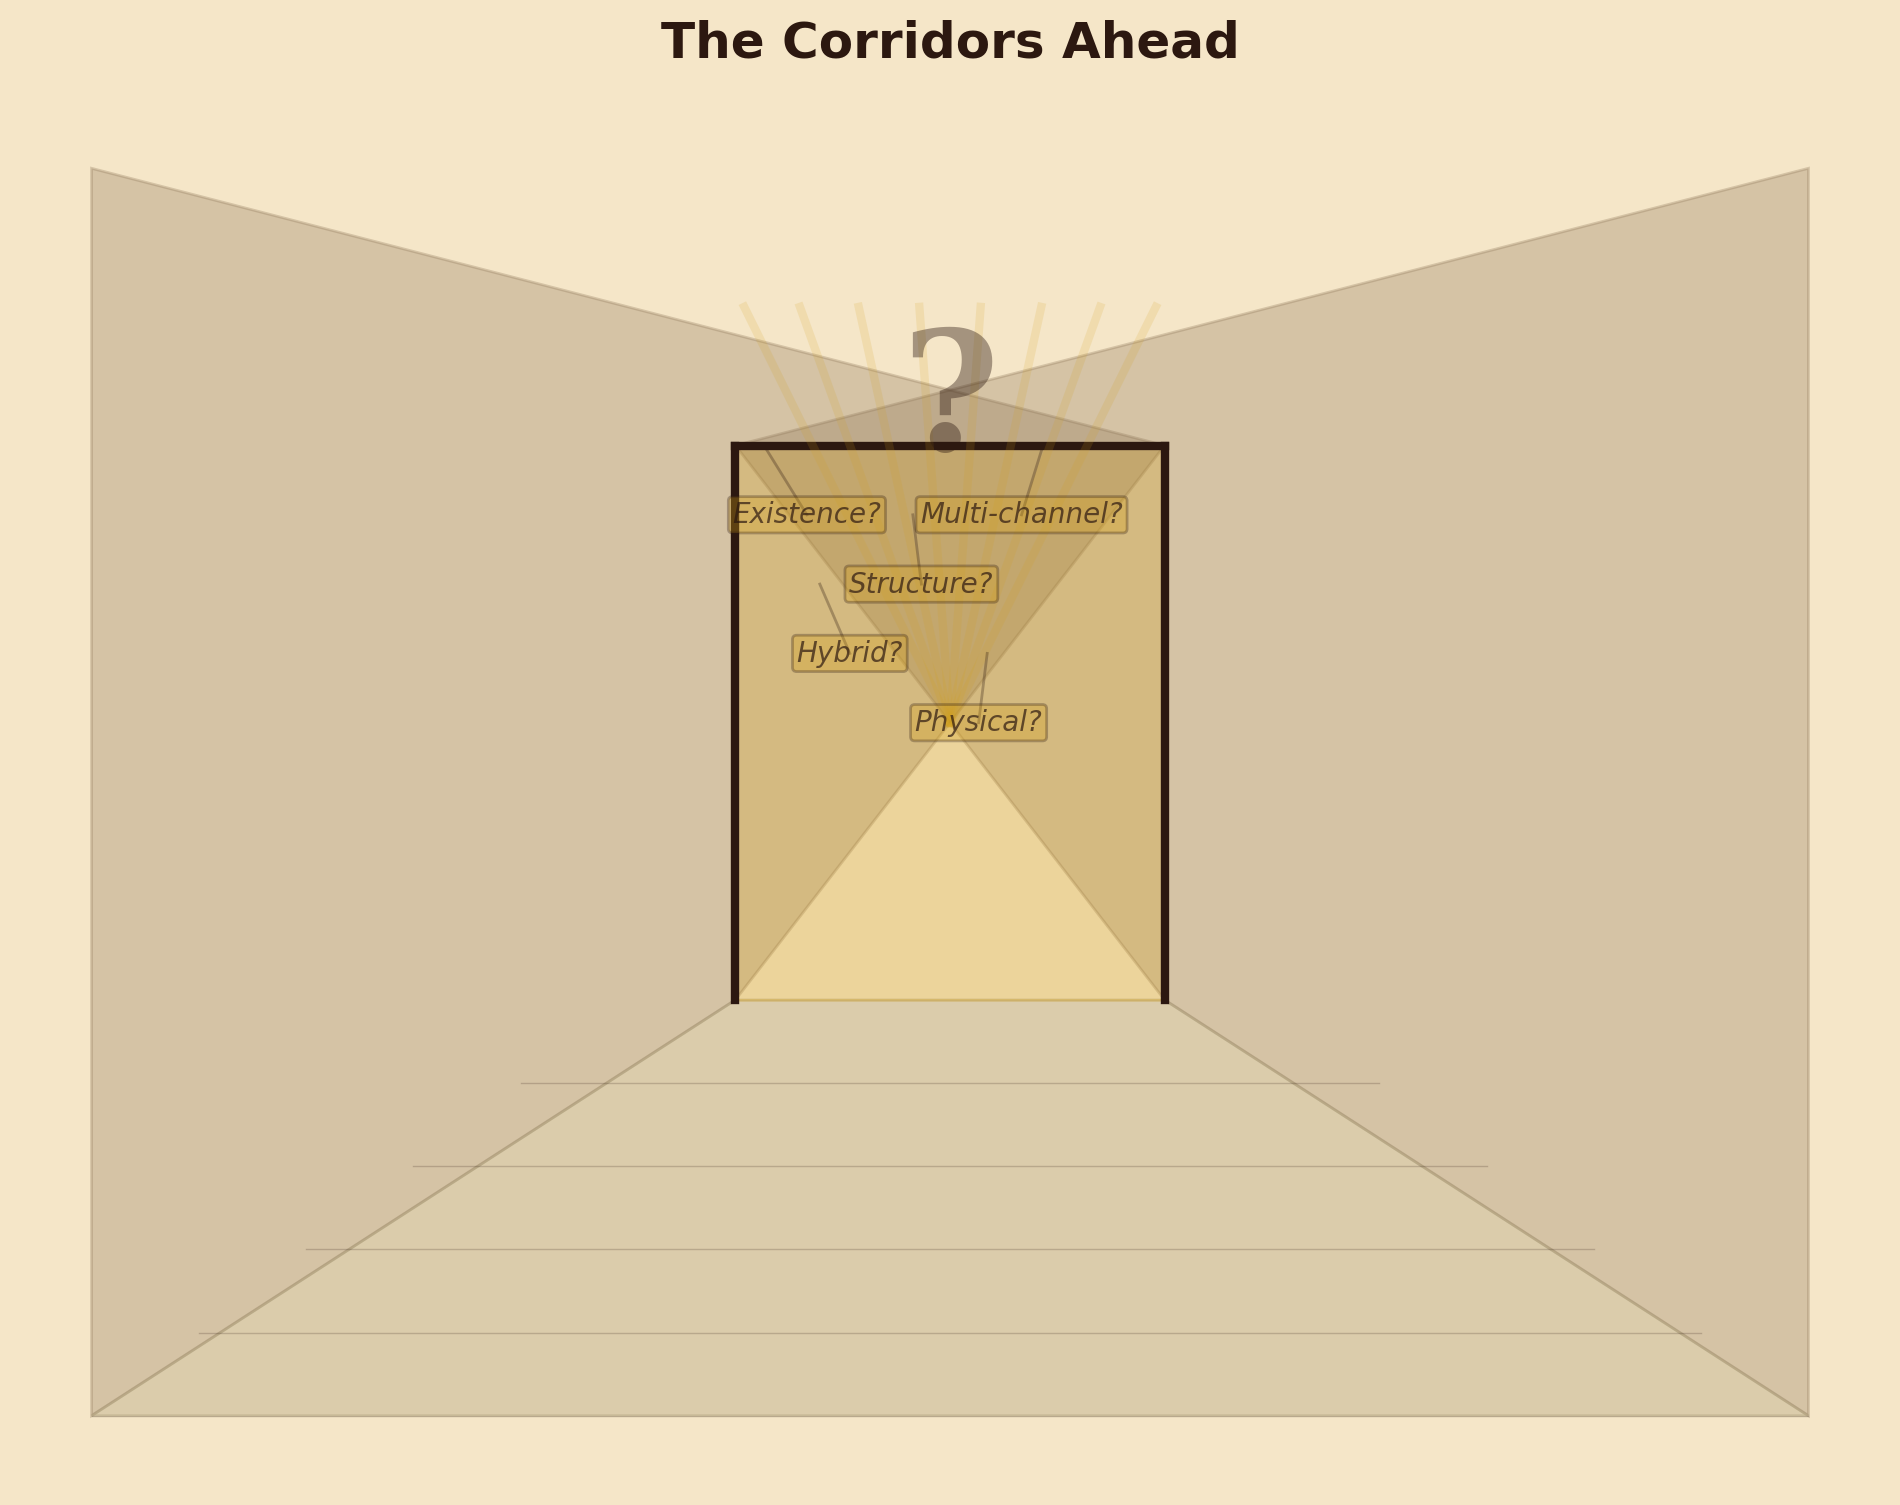
\includegraphics[width=0.82\textwidth]{../Chapter7/images/fig12_corridors_ahead.png}
\caption{An open doorway at the end of a stone corridor, with warm sunlight streaming through. Through the doorway, a vista of many more branching corridors is visible, stretching into the distance, each\ldots}
\end{figure}


\bigskip


\textit{In the next chapter, we shall leave the corridors of the Pythagorean tree and step into a different labyrinth entirely --- one built not from right triangles but from the algebra of octonions, where the rules of multiplication themselves become a source of mathematical wonder.}
\index{octonions}

